\documentclass[a4paper,12pt]{report}
\setcounter{secnumdepth}{5}
\setcounter{tocdepth}{3}
\newcounter{ZhRenew}
\setcounter{ZhRenew}{1}
\newcounter{SectionLanguage}
\setcounter{SectionLanguage}{1}
\input{/usr/share/latex-toolkit/template.tex}
\begin{document}
\title{大氣科學與海氣交互作用}
\author{沈威宇}
\date{\temtoday}
\titletocdoc
\chapter{大氣科學(Atmospheric Science)與海氣交互作用(Air-Sea Interaction )}
\section{對流層大氣(Tropospheric atmosphere)/空氣(Air)的成分}
\begin{itemize}
\item 對流層大氣中,水氣約占0至5\%,其餘中,氮氣約占78.08\%,氧氣約占20.95\%,氬氣約占0.93\%,二氧化碳約占0.04\%。水氣、二氧化碳、甲烷、臭氧、氮氧化物、硫氧化物等比例變動率較大,稱變動氣體。STP 密度 1.293 kg/m$^3$,NTP 密度 1.204 kg/m$^3$。
\item 對流層大氣中,水氣、二氧化碳、甲烷等溫室氣體,吸收長波輻射,維持地表溫度。
\item 對流層大氣中有氣懸膠體,指其中懸浮的固體和液體微粒,可作為凝結核。
\end{itemize}
\section{氣壓垂直變化}
\ssc{大氣壓力/氣壓}
單位面積上,由某一高度到大氣層頂空氣柱的總重量。
\ssc{壓力的單位}
\[1\text{\ atm}=1013.25\text{\ hPa}=101325\text{\ Pa}=101325\text{\ N m}^{-2}=1.01325\text{\ bar}=760\text{\ Torr}\]
\[1\text{\ mmHg}=0.1\text{\ cmHg}=1\text{\ mm}\cdot 13595.1\text{\ kg m}^{-3}\cdot 9.80665\text{\ m s}^{-2}=133.322387415\text{\ Pa}\approx 1\text{\ Torr}\]
\[1\text{\ cm\ce{H2O}}=1\text{\ cm wg}=10\text{\ mm\ce{H2O}}=1\text{\ cm}\cdot 1000\text{\ kg m}^{-3}\cdot 9.80665\text{\ m s}^{-2}=98.0665\text{\ Pa}\]
\subsection{氣壓公式(Barometric formula)}
\[P=\begin{cases}
P_b\left(1-\frac{L}{T_b}(h-h_b)\right)^{\frac{gM}{RL}},\quad & L\neq 0,\\
P_be^{-\frac{gM(h-h_b)}{RT_b}},\quad & L=0,
\end{cases}\]
where
\begin{itemize}
\item $P$: pressure at which pressure is calculated
\item $P_b$: reference pressure
\item $T_b$: reference temperature
\item $L$ temperature lapse rate, assumed constant
\item $h$: geopotential height at which pressure is calculated
\item $h_b$: geopotential height of reference level
\item $R$: gas constant, assumed air is ideal gas
\item $g$: gravitational acceleration, assumed constant 
\item $M$: molar mass of air, assumed constant 
\end{itemize}
高度 5.5 km處氣壓約 500 hPa,高度 9 km處氣壓約 300 hPa,高度 50 km處氣壓約 1 hPa,即千分之九百九十九的大氣都在平流層及以下。
\subsection{氣壓高度}
在接近海平面處,高度每增加10公尺,氣壓約降低1百帕。飛機使用氣壓高度確保飛機間高度間距。登山使用的高度計使用氣壓高度原理。
\section{氣溫垂直變化與大氣分層}
地球的大氣層是因地球引力束縛而聚攏在地表(陸地及海洋)周圍的一層氣體混合物,其中還懸浮有不定量的氣膠和顆粒物。地球大氣層根據氣溫垂直遞減率從裡向外可以分為對流層、平流層(同溫層)、中氣層、增溫層和外氣層五個區域,沒有確切的上界。 
\bct\bfH\ctr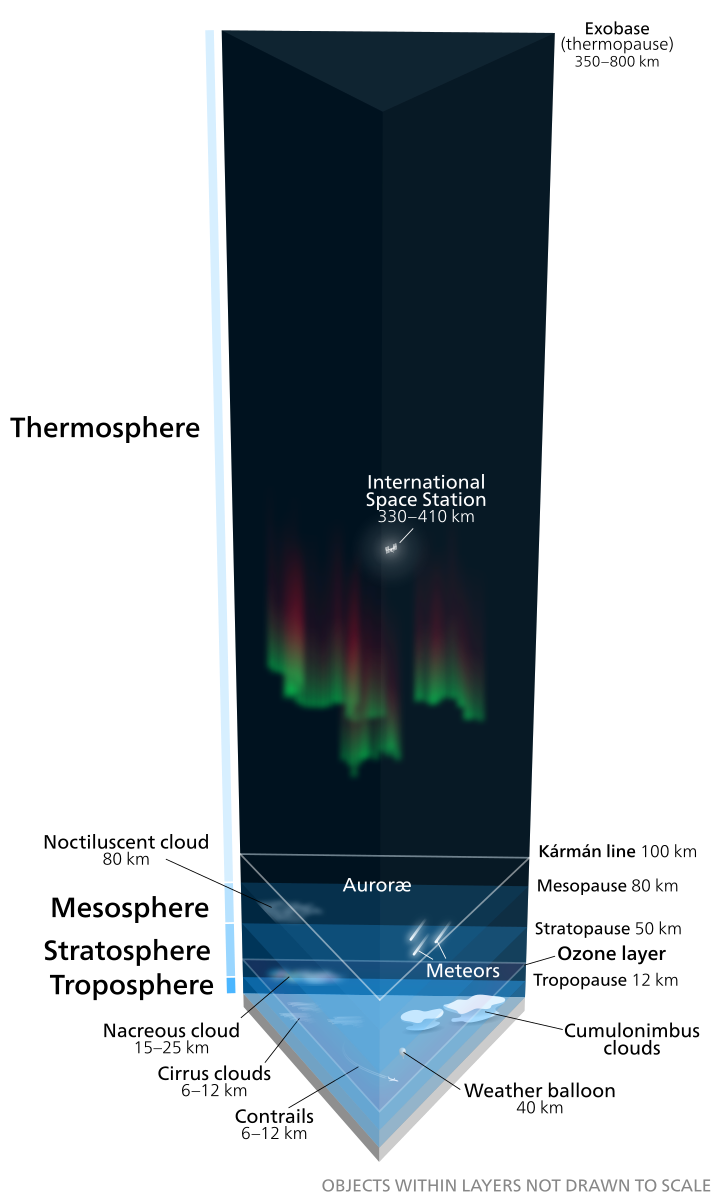
\includegraphics[height=0.8\textheight]{atmosphere.png}\caption{Kelvinsong, 2013}\ef\FB\ect
\subsection{對流層(Troposphere)}
\begin{itemize}
  \item 對流層是地球大氣圈中最底部的一層,下與地面相接,上至平流層。
  \item 對流層上界隨緯度、季節而變化,通常約8\sim 16千米,平均10\sim 12千米,低緯度地區平均約15\sim 17千米,中緯地區平均約10\sim 12千米,高緯地區平均約8\sim 9千米,夏季厚冬季薄,在中緯地區尤甚。
  \item 對流層集中了整個大氣層約75\%的質量,及90\%以上的水及雜質,是密度最高的一層。對流層空氣垂直對流旺盛,天氣現象均發生在此。
  \item 除局部局時的逆溫層外,對流層氣溫直減率為正,平均約6.5攝氏度每公里。對流層頂的溫度約在攝氏-50至-65度。
  \item 太陽輻射中能量最強的可見光基本不能被大氣吸收,而是直接 透過大氣射向地面;地面一邊吸收熱量一邊也向外輻射紅外線,這部分紅外線能量的75\%\sim 95\%都被對流層的溫室氣體等物質吸收截留,是對流層的主要熱源。
  \item 對流:通常發生在流體內或流體和其他物質之間有溫度差時,因為溫度的差異會使得流體之間的密度不同,當流體增溫、體積膨脹、密度變小, 便會逐漸上升,其位置由周圍溫度較低、密度較大的物質補充,補充之物質再增溫上升,周圍物質又來補充,如此循環不已,遂將熱量經流體之流動傳播到各處。
\end{itemize}
\subsection{平流層(Stratosphere)}
\begin{itemize}
  \item 平流層位於對流層上方和中間層下方,其下界即對流層上界, 依緯度、季節而變;其上界距地面50\sim 55km。
  \item 因為以臭氧吸收的熱量為主要熱源,平流層的氣溫直減率大體為負,至平流層頂達約-3℃。
  \item 因為呈現逆溫分布,空氣大多維持水平方向運動。
  \item 等溫層/同溫層(Isothermal layer):平流層在對流層頂至臭氧層底處存在一個溫度垂直變化較小的等溫層。平流層又稱同溫層源於此 。
  \item 臭氧層(Ozone layer):平流層的主要熱源為臭氧直接吸收太陽0.2至0.3微米的紫外線輻射而增溫(更短波長者幾乎已在其上吸收盡)。平流層聚集了大氣層中約90\%的臭氧,臭氧濃度 高值區稱臭氧層,約在距地表20\sim 25千米處。臭氧層可以屏蔽來自地球外的大部分紫外線(幾乎全部的UV-C和大部分UV-B)。
  \item 長程客機注意飛行於平流層底部。
\end{itemize}
\subsection{中性層}
地球大氣層未被電離的部分,包含對流層和平流層。
\subsection{中氣層(Mesosphere)}
中氣層下方是平流層,上方是增溫層,頂部高度約85km。

中氣層臭氧分子稀少,難以吸收太陽輻射,因此氣溫直減率為正,故其中空氣存在相當的垂直方向運動。中氣層底的溫度約-3°C,中氣層頂的溫度約-90至-100°C。
\subsection{均勻層}
地球大氣中各種氣體分子分布均勻的層,包含對流層、平流層與中氣層 。
\subsection{增溫層(Thermosphere)}
增溫層位於中氣層之上及外氣層之下,其頂部離地面約600km。
\begin{itemize}
\item 空氣非常稀少,吸收少許太陽輻射就會大幅升溫,因此溫度隨高度增加而遞增,但密度極低,無法用一般溫度計測量。
\item 溫度約已高於攝氏零度且空氣密度低,故通常在增溫層的航空器不能使用一般飛機的渦輪引擎。
\item 吸收主要來自太陽的<0.2微米短波輻射,主要包含短波紫外線與X射線,是其主要熱源。
\item 大量帶電粒子碰撞可能形成極光。
\end{itemize}
\subsection{卡門線(Kármán line)}
海拔100公里線,被提出為大氣層和太空的分界線,但並未受到全體接受,國際法未定義大氣層和太空的分界。
\subsection{電離層(Ionosphere)}
電離層是地球大氣層被太陽風、宇宙射線等電離的部分,電離指氣體的電子被遊離形成正離子與自由電子。電離層是地球磁層的內界。白天時包含中氣層和增溫層,晚上時僅包含增溫層。
\begin{itemize}
  \item D層:D層是電離層最低的一層,離地球表面50至100公里。這裡主要是波長為121.5奈米的來曼-α氫光譜線的光電離一氧化氮。在太陽活動非常強烈時(超過50個黑子),硬X射線還可以電離空氣中的氮氣和氧氣的分子。白天時方存在,太陽活動愈強愈明顯。
  \item E層:E層是中層,在地面上100至150公里。這裡的電離主要是 軟X射線和遠紫外線對氧氣分子的電離。這個層只能反射頻率低於10MHz 的電波,對頻率高於10MHz的電波它有吸收的作用。夜間E層較不顯著且 高度較高。
  \item E$_\text{s}$層:又稱偶現E層。它是小的、強烈電離的雲,可以反射頻率在25至225MHz之間的電波,可以持續數分鐘到數小時不等。 夏季偶現E層出現得比較多,持續時間一般也比冬季長。電波的反射距離一般為1000公里左右。
  \item F層:F層在地面以上150至超過500公里。在這裡太陽輻射中的 強紫外線(波長10至100奈米)電離單原子氧。F層對於電波傳播來說是 最重要的層。夜間F層合併為一個層,白天分為F$_1$和F$_2$兩個層。大多數無線電波天波傳送是F層形成的。在白天F層是電離層反射率最高的 層。
\end{itemize}
\subsection{外氣層(Exosphere)/散逸層}
位於增溫層的上方,沒有明確上界。溫度極高, 空氣粒子運動很快,經常散逸至外太空。
\subsection{不均勻層}
地球大氣中各種氣體分子分布不均勻的層,包含增溫層及以上。
\subsection{氣溫垂直遞減率(Lapse rate of temperature)}
\begin{itemize}
  \item 氣溫垂直遞減率簡稱氣溫直減率。是氣溫隨著高度上升而遞減的幅度。
  \item 空氣是熱的不良導體,因此空氣團垂直移動的過程可以視為絕熱膨脹(絕熱降溫、絕熱冷卻)與絕熱壓縮(絕熱升溫、絕熱增溫)。 一般稱絕熱乾空氣團溫度隨高度上升而遞減的幅度為乾絕熱直減率,稱絕熱溼空氣團溫度隨高度上升而遞減的幅度為溼絕熱直減率。空氣團上升過程中,體積增加,故絕對溼度減少,但溫度下降,故相對溼度增加除非飽和。
  \item 在對流層中,除局地局時的逆溫層外,氣溫直減率大於零;乾空氣平均每上升100公尺,氣溫就下降約0.98度;溼空氣因為水氣凝結時會釋放潛熱,平均每上升100公尺,氣溫下降約0.60度;平均空氣平均每上升100公尺,氣溫下降約0.65度。
\end{itemize}
\section{大氣與地表能量收支}
\bct\bfH\ctr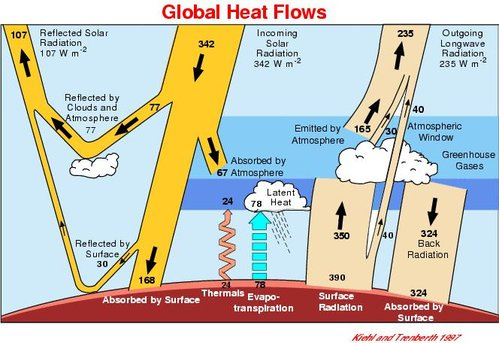
\includegraphics[width=0.9\textwidth]{heat_flow.jpg}\caption{Trenberth (2020) Journal of the Royal Society of New Zealand, 50:2, 331-347. c The Royal Society of New Zealand}\efct
\begin{itemize}
  \item 太陽輻射是地球最主要的外部能量來源,也是推動大氣運動及 天氣變化的主要能量。太陽輻射進入地球大氣後,部分會被大氣(氣體 分子、懸浮微粒、雲等)吸收,部分會被大氣反射,約一半達到表,達 到地表者少部分被地表反射,大部分被地表吸收。
  \item 地球的能量支出部分,主要是透過地表紅外線輻射持續向外發 散能量,絕大部分的地表紅外線輻射會被大氣中的溫室氣體吸收,小部 分會直接逸散到太空。
  \item 大氣的能量也會以紅外線輻射的形式,發射至地表與太空。
  \item 空氣對流與水蒸發的潛熱也會將能量向上帶。
  \item 溫室效應(Greenhouse effect):大氣氣體吸收來自太陽或行星的輻射能量,再輻射給行星的效應。溫室效應在白天由大氣吸收地表 輻射較多,晚上由地表吸收大氣輻射較多,使行星表面晝夜溫差較小。
  \item 地球總反照率約31\%。
\end{itemize}
\section{大氣的水氣變化}
\subsection{絕對溼度}
單位體積空氣中所含的水蒸氣質量,通常單位g/m$^3$。
\subsection{相對溼度}
指實際水氣壓(即水蒸氣在空氣中的分壓)除以水在該溫度的飽和蒸氣壓。一般70\%的相對溼度對人體而言較舒適,低於50\%會感覺乾燥。
\subsection{露點(溫度)(Dew point)}
露點或露點溫度指在固定氣壓和水氣壓下,空氣中所含的氣態水達到飽和而凝結成液態水所需要降至的溫度。
\subsection{大氣穩定度}
大氣穩定度決定當空氣塊抬升條件消失後空氣塊會繼續上升、停留不動還是下沉返回地表。
\begin{itemize}
  \item 絕對穩定:環境直減率$\leq$6°C/km,空氣團上升後會降溫到比外界低溫而下降,大氣不易有垂直對流,若外力足以抬升其到凝結高度以上則生成積雲,但因失去外力抬升即下沉故不利雲系向上發展。
  \item 絕對不穩定:環境直減率$>$10°C/km,空氣團上升後仍比外界高溫而繼續上升,冷空氣下降填補其位置,大氣易有垂直對流,抬升條件消失後相對外界輕的空氣塊繼續上升形成易向上發展的積雨雲。
  \item 條件不穩定/相對穩定:環境直減率$>$6°C/km且$\leq$10°C/km,溼空氣團上升後會降溫到比外界低溫而下降,不易有垂直對流;乾空氣團上升後仍比外界高溫而繼續上升,冷空氣下降填補其位置,易有垂直對流;即要有迫使空氣塊抬升至特定高度的條件發生,大氣穩定度才會發生改變。
\end{itemize}
\subsection{成雲致雨}
空氣絕熱上升冷卻,造成相對溼度上升,達到露點,水氣遂凝結為水,若降溫至熔點以下,水就可能凝固成冰晶,係成雲致雨的重要機制。
\sssc{凝結核}
是懸浮於空氣中的微粒,能幫助水氣於其上凝結成小水滴,可以說固態、液態或兩者之混合物。凝結核的成分多樣,高空卷雲的凝結核通常是冰核,其他凝結核則可分為不可溶但能為水溼潤的粒子,如沙、塵埃,以及可溶性的鹽粒,如硫酸鹽、硝酸鹽。若空氣十分純淨而無凝結核,則不易成雲致雨。
\sssc{冰核}
與凝結核相似,水凝固為冰晶也需要冰核,缺乏冰核時可能低於熔點仍未結冰,稱過冷水。大氣中的冰核數量遠少於凝結核,故高空雲層中常有過冷水。當過冷水遇到冰核會迅速凝固,如通過雲層的飛機,可能會因機身結冰造成危險。
\sssc{空氣抬升與降雨方式}
\begin{itemize}
\item 局部熱對流抬升與對流雨:地面空氣受較暖地表或海面加熱,密度變小而產生強烈的上升氣流,造成對流雲系發展而降雨,並伴隨閃電。如夏季午後的雷陣雨。
\item 地形抬升與地形雨:氣流在迎風坡順地勢抬升,在迎風面成雲致雨,通常不伴隨閃電;在背風面可能因水氣不飽和氣流下沉升溫出現乾熱的焚風(Foehn)/火燒風。焚風係因氣團中水氣已在迎風坡降水用盡,氣團絕熱下降溫度升高,故特徵為相對於原本該地氣團而言氣溫顯著上升、露點通常下降。如臺灣北部與東北部在冬季為東北季風迎風坡而降雨、颱風或低壓系統通過臺灣東北部時南臺灣吹西風常在臺東一帶形成焚風。
\item 鋒面抬升與鋒面雨:冷暖氣團交會時,密度較小的暖氣團沿鋒面抬升成雲致雨。如冬、春兩季冷鋒通過臺灣帶來降雨。
\item 幅合抬升與幅合雨:低氣壓中心低層空氣向內輻合,迫使空氣向上運動,易形成陰雨天氣。如熱帶低氣壓或颱風帶來的雨。
\end{itemize}
\sssc{人工降雨(Cloud seeding)}
\begin{itemize}
\item 地面造雨法:利用地面造雨器燃燒碘化銀溶液,使碘化銀煙粒隨熱氣飄升達高空過冷水滴層以充當凝結核,使過冷水滴凝固為冰晶,經由冰晶成長過程,終至掉落成雨。
\item 空中造雨法:利用飛機在雲中撒播碘化銀或乾冰雲種,由於撒播之雲種可精確被送達足夠低溫之雲中,故一般造雨效果較佳。
\end{itemize}
\subsubsection{霧}
雲霧成因相同,都是空氣因冷卻而達飽和而凝結或凝固的現象,高空者稱雲,近地面或海面的稱霧。

霧附著於表面呈液態者稱露,呈固態者稱霜。
\begin{itemize}
\item 輻射霧:地表向外輻射熱能於白天小於吸收之熱能,晚上則大於之,使溫度下降,待水氣達到飽和所形成的霧,多出現於清晨,而消散於太陽出來後。
\item 平流霧:暖溼空氣在寒冷的陸地或海面上平流,使流動的空氣冷卻凝結,渦流混合可使此飽和空氣的霧滴伸展至相當高度,出現時間不固定。
\item 升/上坡霧/膨脹霧:指因為地形使冷空氣抬升,因絕熱膨脹而冷凝而產生的霧。
\item 蒸氣霧:冷空氣通過溫暖的水面,獲得來自水面的足夠水氣而飽和,常見於高緯度、秋冬交際的河面或湖面。
\item 鋒面霧:暖空氣沿鋒面抬升降雨,雨滴落下後又蒸發,使下層冷空氣飽和生霧。
\end{itemize}
臺灣常見輻射霧與平流霧。冬末春初之晴天晚上,臺灣西部因暖溼空氣流入與輻射冷卻雙重影響,在清晨出現能見度不到百米的大霧。
\section{大氣的水平運動}
在地球參考系觀察,空氣所受的力主要有:氣壓梯度力、旋轉參考系的假想力、重力、摩擦力等。
\subsection{地球上的科里奥利力/科氏力(Coriolis force)}
地球參考系是一個旋轉參考系,地球自轉角頻率$\omega$即地球參考系相對於慣性參考系的角頻率,其中物體存在離心力(Centrifugal force)、科里奥利力/科氏力(Coriolis force)與尤拉力(Euler force)三個假想力。緯度$\phi$處一質量$m$、速度$\mb{v}$質點相對於地球所受科氏力$\mathbf{F}_c$為:
\[ \mathbf{F}_c = -2m\omega \mathbf{v} \sin \phi \]
\(f = 2\omega \sin \phi\) 稱科氏參數(Coriolis parameter)/科氏頻率(Coriolis frequency)。科氏力會使北半球的物體在飛行途中向右轉,南半球的物體在飛行途中向左轉。
\subsection{氣壓梯度力(Pressure Gradient Force, PGF)}
氣壓作為一個純量場,其梯度稱氣壓梯度,因為氣壓差造成的力稱氣壓梯度力。等壓線指氣壓相等處的連線。等壓線疏密程度與氣壓梯度呈正比。
\[ \mathbf{F}_p = -\frac{1}{\rho} \nabla p \]
其中 $\mathbf{F}_p$ 是氣壓梯度力,\(\rho\) 是空氣密度,\(p\) 是氣壓。
\subsection{空氣的運動}
\begin{itemize}
  \item 空氣的垂直運動:因為向上的氣壓梯度力分量與向下的重力大 致相等達到平衡,因此空氣的垂直運動速度很小,每秒僅約速公分。但 當積雨雲發展或劇烈天氣現象發生時空氣垂直運動速度可以很大,例如 下雷雨時雲內的垂直速度可達每秒數十公尺。
  \item 風:風是指空氣的水平運動,速度一般每秒約數公尺。
  \item 風向:風的來向。
\end{itemize}
\subsection{蒲福風級(Beaufort scale)}
1805年英國海軍上將蒲福建立,原用於海上,後屢經修訂,乃成今日通用之風級。
\bctf
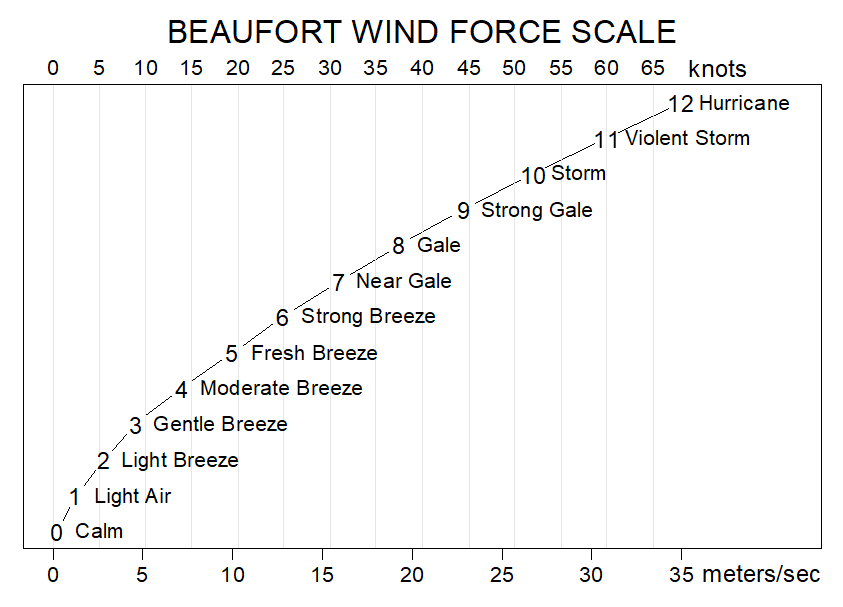
\includegraphics[width=0.9\textwidth]{Beaufort_wind_scale.png}\caption{Ldecola, 2018}
\efct
\subsection{風切(Wind shear)}
註:此處將空氣向任何方向的運動視為風。

令向東、向北和向上分別為 \(x\)、\(y\) 和 \(z\) 方向。風向量場可以表示為:\(\mathbf{V} = (u, v, w) \),其中 \(u\)、\(v\) 和 \(w\) 分別表示在 \(x\)、\(y\) 和 \(z\) 方向的風速分量。

風切的數學描述:可以用風向量場的空間變化率來描述,即風向量場的梯度張量 \(\nabla \mathbf{V}\):
\[ \nabla \mathbf{V} = \begin{pmatrix} \frac{\partial u}{\partial x} & \frac{\partial u}{\partial y} & \frac{\partial u}{\partial z} \ \frac{\partial v}{\partial x} & \frac{\partial v}{\partial y} & \frac{\partial v}{\partial z} \ \frac{\partial w}{\partial x} & \frac{\partial w}{\partial y} & \frac{\partial w}{\partial z} \end{pmatrix} \]
\subsection{地轉風(Geostrophic wind)}
地轉風是一種科氏力和氣壓梯度力平衡(稱地轉平衡)下產生的理論上的風,方向和等壓線平行。
  \begin{itemize}
    \item 假設大氣處於平衡狀態,即不考慮加速度;假設風是水平的 ,即忽略垂直運動;假設空氣運動不受摩擦力影響;假設風向量場是連 續的。
    \item 推導:
    \[ \mathbf{F}_c = -2\Omega \mathbf{v} \sin \phi \]
    其中 $\mathbf{F}_c$ 是科氏力,\(\Omega\) 是地球的自轉角速度,\(\mathbf{v}\) 是風速向量,\(\phi\) 是緯度。
    \[ \mathbf{F}_p = -\frac{1}{\rho} \nabla p \]
    其中 $\mathbf{F}_p$ 是氣壓梯度力,\(\rho\) 是空氣密度,\(p\) 是氣壓。
    \item 地轉平衡
    在地轉平衡條件下,氣壓梯度力與科氏力平衡,即:
    \[ \mathbf{F}_p + \mathbf{F}_c = 0 \]
    代入上述表達式:
    \[ -\frac{1}{\rho} \nabla p - 2\Omega \mathbf{v} \sin \phi = 0 \]
    將 \(\mathbf{v}\) 表示為風速的分量 \((u, v)\),在北半球:
    \[ -\frac{1}{\rho} \frac{\partial p}{\partial x} - 2\Omega v \sin \phi = 0 \]
    \[ -\frac{1}{\rho} \frac{\partial p}{\partial y} + 2\Omega u \sin \phi = 0 \]
    重新整理上述方程:
    \[ u = -\frac{1}{2\Omega \sin \phi \rho} \frac{\partial p}{\partial y} \]
    \[ v = \frac{1}{2\Omega \sin \phi \rho} \frac{\partial p}{\partial x} \]
    將空氣密度 \(\rho\) 替換為標準大氣密度,並簡化得:
    \[ u = -\frac{1}{f} \frac{\partial p}{\partial y} \]
    \[ v = \frac{1}{f} \frac{\partial p}{\partial x} \]
    其中,\(f = 2\Omega \sin \phi\) 是科氏參數。
    \item 最終表達式
    \[ \mathbf{v}_g = \left( -\frac{1}{f} \frac{\partial p}{\partial y}, \frac{1}{f} \frac{\partial p}{\partial x} \right) \]
    這說明地轉風速度的大小和方向取決於氣壓梯度和緯度(通過科氏參數 \(f\))。在北半球,地轉風平行於等壓線,氣壓梯度力指向低壓區,風向與氣壓梯度力成90度角,右側為高壓,左側為低壓;在南半球 ,方向相反。
\end{itemize}
\ssc{地轉風近地面風}
\begin{itemize}
  \item 大氣和地表的摩擦力破壞了地轉平衡。摩擦力使氣流速度降低 ,減弱了科氏力的效果。結果就是氣壓梯度力效果變大,造成更大的偏 轉讓空氣持續從高氣壓流往低氣壓。這解釋了為什麼高氣壓系統的風持 續從中心向外,而低氣壓系統的風則是螺旋向系統中心。
  \item 高空風(地轉風):通常,離地約1公里以上的高空風接近地轉風。
  \item 近(陸地)地面風:陸地地表摩擦力較大,風向較地轉風接近 氣壓梯度力,斜向穿過等壓線,與等壓線夾約15\sim 30°,風速較高空地轉 風小。
  \item 近海面/冰面風:海面與冰面摩擦力遠小於陸地,風向較近陸地地面風更接近地轉風。
  \eit
\subsection{高氣壓與低氣壓}
高氣壓又稱反氣旋,低氣壓又稱氣旋。在北半球,高壓中心近地面的空氣,會以順鐘向向外輻散,中心區域空氣下沉,水氣不易上升凝結,故多為晴朗天氣;低壓中心近地面的空氣,會以逆鐘向向內輻合,中心區域空氣上升,水氣易上升凝結,故多為陰雨天氣;南半球旋向反之。

龍捲風因尺度較小不受科氏力影響。
\section{大氣系統(Atmospheric system)}
\subsection{大氣系統的尺度}
尺度指一事件所涵蓋的空間與時間大小,兩者正相關。
\begin{itemize}
\item 行星尺度(Planetary scale): 如行星風系、沃克環流。
\item 縱觀尺度(Synoptic scale):水平範圍2000公里以上。如氣團、部分鋒面(滯留鋒常見)、部分寒、溫、熱帶氣旋、少數海陸風。
\item 中尺度:水平範圍20至2000公里。如部分海陸風、山谷風、焚風、部分雷雨、部分龍捲風、部分沙塵暴。
\item 小尺度:水平範圍不足20公里。如部分雷雨、部分龍捲風、部分沙塵暴、小型渦流。
\end{itemize}
\subsection{大氣環流(Atmospheric circulation)的原因}
當地球受熱不均,冷處較暖處密度較大,故垂直地表方向等壓線較密集,故在地面冷處形成高氣壓,暖處形成低氣壓,前者氣流地面輻散、高空輻合,後者反之,共形成一環流。
\subsection{海氣交互作用(Air-sea interaction )}
大氣與海洋同為流體,兩者間有物質與能量交換,稱海氣交互作用。

海氣間熱量傳遞:
\begin{itemize}
\item 潛熱:海水比熱較高,能保存較多熱能,可能透過蒸發散作用傳播給大氣,乾燥高溫海域尤甚,在多數海域長期平均潛熱通量為正(指海洋放熱給大氣),且約緯度愈低愈大,太平洋赤道一帶約120至160瓦每平方米,極區接近零,亦受海流影響。臺灣至日本本州一帶因西太平洋暖水區/暖池(Western Pacific Warm Pool)與黑潮暖流,且北半球陸地面積較大使太平洋間熱帶輻合區在赤道之北,故極大,可達150至200瓦每平方米;秘魯湧升流一帶因湧升流較冷,故極小,可達接近零。
\item 顯熱:熱量直接由高溫介質傳導至低溫介質,較潛熱通量小,亦受緯度與海流影響,多數非沿海海域在-10至20瓦每平方米之間。臺灣至日本本州一帶極大,可達40至60瓦每平方米。
\end{itemize}
\subsection{鋒(Front)/鋒區/鋒面}
氣象學上的鋒或鋒區是指具有強水平溫度梯度、較大靜力穩定性及較大氣旋性渦度的狹長地帶,出現在兩個密度不同的氣團之間。其寬約數十或數百千米,長約上千千米,屬於中尺度天氣系統。鋒在天氣圖上表現隨高度向冷區傾斜的等溫線密集帶。鋒面通過時,造成空氣抬升,地面在鋒面所在處形成暫時低壓區,而氣團多為高氣壓,故鋒面通過時較鋒面通過前後氣壓低。天氣圖上鋒面的位置繪製於地面兩氣團分界之處。鋒面造成兩氣團中較暖者抬升至較冷之上深入之,故可能於該區域發生成雲致雨,對冷鋒而言為鋒後,對暖鋒而言為鋒前。
\subsubsection{伯傑龍氣團分類(Bergeron classification of air masses)}
The Bergeron classification of air masses is a system used in meteorology to classify air masses based on their source region and moisture content. It was developed by Swedish meteorologist Tor Bergeron in the early 20th century. The classification uses three main letters to describe an air mass.
\begin{itemize}
\item Moisture Content: first, lowercase letter
\begin{itemize}
\item c: Continental (dry air)
\item m: Maritime (moist air)
\end{itemize}
\item Thermal Characteristics: second, uppercase letter
\begin{itemize}
\item P: Polar (cold air from higher latitudes)
\item T: Tropical (warm air from lower latitudes)
\item A: Arctic (very cold air from the Arctic region)
\item E: Equatorial (hot, humid air from near the equator)
\item S: Superior air (dry air formed by significant downward motion in the atmosphere)
\end{itemize}
\item Surface Modifiers: optional third, lowercase letter
\begin{itemize}
\item k: Indicates the air mass is colder than the surface it moves over (e.g., causes instability and convection).
\item w: Indicates the air mass is warmer than the surface it moves over (e.g., causes stability).
\end{itemize}
\end{itemize}
\subsubsection{冷鋒(Cold front)}
冷氣團主導向暖氣團推進,並取代暖氣團原有位置所形成的鋒。因為冷氣團密度大於暖氣團,故移動速度較暖鋒快。由於冷氣團的密度較暖氣團大,相遇時冷氣團會下沉到暖氣團的下方,暖氣團被迫抬升。在上升過程中,空氣逐漸冷卻,形成雲層,若暖氣團中含有大量的水分,就會形成降水,發生在鋒後。因冷鋒鋒面較陡,易形成向上堆疊的積雲,鋒區所在的低壓槽較暖鋒窄,故降雨範圍較暖鋒窄,通常為降雨強度較大的間歇性降雨。

臺灣冷鋒通常發生在冬、春兩季。
\bct
\begin{figure}[H]
\centering
\begin{tabular}{|p{0.1\textwidth}|p{0.25\textwidth}|p{0.25\textwidth}|p{0.25\textwidth}|}
\hline
氣象要素 & 過境前 & 過境時 & 過境後 \\ \hline
風向 & 偏南或偏西南 & 快速變化 & 偏西或偏西北 \\ \hline
溫度 & 相對較高 & 急劇下降 & 穩定下降 \\ \hline
氣壓 & 穩定下降 & 達到最低值後急劇上升 & 穩定升高 \\ \hline
雲系 & 捲雲和卷層雲增多,臨近過境時出現積雨雲 & 積雨雲 & 積雲為主,地面溫度較高時可能有層積雲出現 \\ \hline
降雨 & 短周期的強降雨 & 以雨或雪等形式出現強降雨,有時伴有冰雹和雷電 & 冷鋒前緣暖空氣堆積,降雨強度減弱,隨後放晴 \\ \hline
露點 & 較高 & 急劇下降 & 較低 \\ \hline
能見度 & 一般或較差,有霧 & 很差,但過境結束後提高 & 降雨結束後相對較好 \\ \hline
\end{tabular}
\caption{北半球冷鋒過境後的典型天氣特徵}
\end{figure}\FB\ect
\subsubsection{暖鋒(Warm front)}
暖氣團主導向冷氣團推進,並取代冷氣團原有位置所形成的鋒。因為暖氣團密度小於冷氣團,故移動速度較冷鋒快。由於冷氣團的密度較暖氣團大,相遇時冷氣團會下沉到暖氣團的下方,暖氣團被迫抬升。在上升過程中,空氣逐漸冷卻,形成雲層,若暖氣團中含有大量的水分,就會形成降水,發生在鋒前。因暖鋒鋒面較緩,易形成層雲,鋒區所在的低壓槽較冷鋒寬,故降雨範圍較冷鋒寬,通常為降雨強度較小的持續性降雨,形成細雨綿綿的天氣。

臺灣通常無暖鋒;日本在春、夏之交常有暖鋒。
\bct
\begin{figure}[H]
\centering
\begin{tabular}{|p{0.1\textwidth}|p{0.25\textwidth}|p{0.25\textwidth}|p{0.25\textwidth}|}
\hline
氣象要素 & 過境前 & 過境時 & 過境後 \\ \hline
風向 & 偏南或偏東南 & 多變 & 偏南或偏西南 \\ \hline
溫度 & 相對較低,緩慢上升 & 穩定上升 & 趨於平穩 \\ \hline
氣壓 & 常為下降 & 急劇下降 & 略微升高後繼續下降 \\ \hline
雲系 & 捲雲和卷層雲增多,隨後出現高層雲、雨層雲和層雲 & 層雲為主 & 放晴,伴有少量層積雲 \\ \hline
降雨 & 輕微到中等程度的降雨 & 零星小雨或無降雨 & 通常無降雨,有時會有小雨或陣雨 \\ \hline
露點 & 穩定升高 & 保持穩定 & 升高後趨於平穩 \\ \hline
能見度 & 很差 & 很差,但逐漸轉好 & 較好,有薄霧 \\ \hline
\end{tabular}
\caption{北半球冬季暖鋒過境前後的典型天氣特徵}
\end{figure}\FB\ect
\subsubsection{滯留鋒/靜止鋒/準靜止鋒(Stationary front)}
指移動緩慢的鋒。滯留鋒兩側的冷暖氣團勢力相當,使鋒在一定區域內來回擺動,造成長時間的晴雨相隔或降雨天氣。冷空氣和暖空氣兩側的風通常幾乎平行於靜止鋒流動,通常沿著靜止鋒兩側以相反的方向流動。通常在地面鋒線過後開始出現降水,風速增大且天氣轉差,待高空槽過境後,降水逐漸停止,天氣開始轉晴。但由於滯留鋒的坡度較冷鋒更小,其雲雨區亦較寬廣,甚至可能使其雲雨區距離地面鋒線較遠。

滯留鋒可能由冷鋒或暖鋒演變而來。

臺灣滯留鋒通常發生在5、6月的梅雨季,長江中下游通常發生於6、7月的梅雨季。當西南氣流與滯留鋒相遇時,導致空氣中的水汽大量凝結,形成持續性的降雨,是梅雨的主要成因。
\subsubsection{囚錮鋒(Occluded front)}
通常是由於冷鋒追上暖鋒而成。在剖面圖上,原來兩個鋒面之間的交接點稱為囚錮點。囚錮鋒的形成經常發生在溫帶氣旋的成熟階段,通常出現在中高緯度地區。當下方被冷空氣占據,暖空氣穩定在上方時,鋒面系統也將消散。
\begin{itemize}
  \item 冷式囚錮鋒:冷鋒後的冷氣團比暖鋒前的冷氣團更冷,其間的 囚錮鋒稱為冷式囚錮鋒。冷式囚錮鋒是由於一個更冷的氣團追上暖鋒, 楔入暖鋒底部而形成。
  \item 暖式囚錮鋒:暖鋒前的冷氣團比冷鋒後的冷氣團更冷,其間的 囚錮鋒稱為暖式囚錮鋒。暖式囚錮鋒是由於冷鋒追上更冷的氣團,冷鋒 被迫抬升所造成的。
  \item 中性囚錮鋒:囚錮鋒前後的冷氣團無太大的差異。
\end{itemize}
\subsection{熱帶氣旋(Tropical cyclone, TC)}
\subsubsection{生成條件}
\bct\bfH\ctr\icg[width=0.9\textwidth]{tropical_cyclone.jpg}\ef\FB\ect
\begin{itemize}
  \item 海面溫度高於26°C(或有稱26.5°C),以提供足夠水氣與能量維持大規模對流結構。
  \item 大氣的初始渦旋:大氣要先有一個低層向中心輻合、高層向外輻散的渦旋,才能維持上升氣流。
  \item 中低對流層的溼度:中低對流層的大氣水氣要充足,才能有更多的潛熱釋放。
  \item 緯度:太接近赤道的地區,地球自轉的科氏力太小,不已形成氣流旋轉與輻合作用,因此在緯度5度以內極少有颱風形成。
  \item 垂直風切小:上下層大氣的風向與風速不能有太大差異 ,才能讓水氣凝結釋放的潛熱集中在熱帶擾動的中心區域。
\end{itemize}
故通常發生在夏季到初秋時分熱帶、副熱帶地區海面,而南大西洋因為溫度較低與風切較大,無熱帶氣旋。
\subsubsection{分級}
\begin{itemize}
  \item 熱帶擾動(Tropical disturbance):中心持續風力未達每小時41公里。熱帶海洋接受較多的太陽輻射,海水溫度較高、蒸發較旺盛 ,潮溼的熱帶大氣獲得充足水氣,得以支持活躍的對流作用。較強對流 產生群聚的積雨雲,環境初始擾動,範圍達數百公里,稱熱帶擾動。
  \item 熱帶低壓/熱帶性低氣壓(Tropical Depression, TD):中心持續風力達每小時41-62公里,即蒲福風級7級。大氣對流開始有組織,四周低層潮溼空氣由周圍向中心輻合、上升,形成高聳的積雨雲,帶來更多水氣與潛熱釋放,被加熱上升後,在高空會形成高壓,使空氣由中心在高層向外輻散,形成之。
  \item 熱帶風暴(Tropical storm, TS)/輕度颱風:中心持續風力達每小時62-117公里,即蒲福風級8-11級,美國稱熱帶風暴(風速1分鐘平均),中華民國稱輕度颱風(風速10分鐘平均)。低壓中心附近上層潛熱釋放,加強對流,更多水氣向低壓中心集中,海面氣壓更低,促使環流加強,吸引更多水氣向低壓中心集中輸送,循環不已,形成之。
  \item 中度與強烈颱風/颱風(Typhoon, TY):西北太平洋稱颱風、大西洋和東太平洋稱颶風(Hurricane)、印度洋及西南太平洋稱旋風(Cyclone)。美國(風速1分鐘平均)每小時118-153公里稱1級颶風、每小時154-177公里稱2級颶風、每小時178-209公里稱3級颶風、每小時210-249公里稱4級颶風 、每小時大於250公里稱5級颶風。中華民國(風速10分鐘平均)每小時118-183公里稱中度颱風,即蒲福風級12-15級、每小時大於184公里稱強烈颱風,即蒲福風級16級以上。此時颱風進一步加強,結構完整。
\end{itemize}
\subsubsection{成熟颱風結構}
\bct\bfH\ctr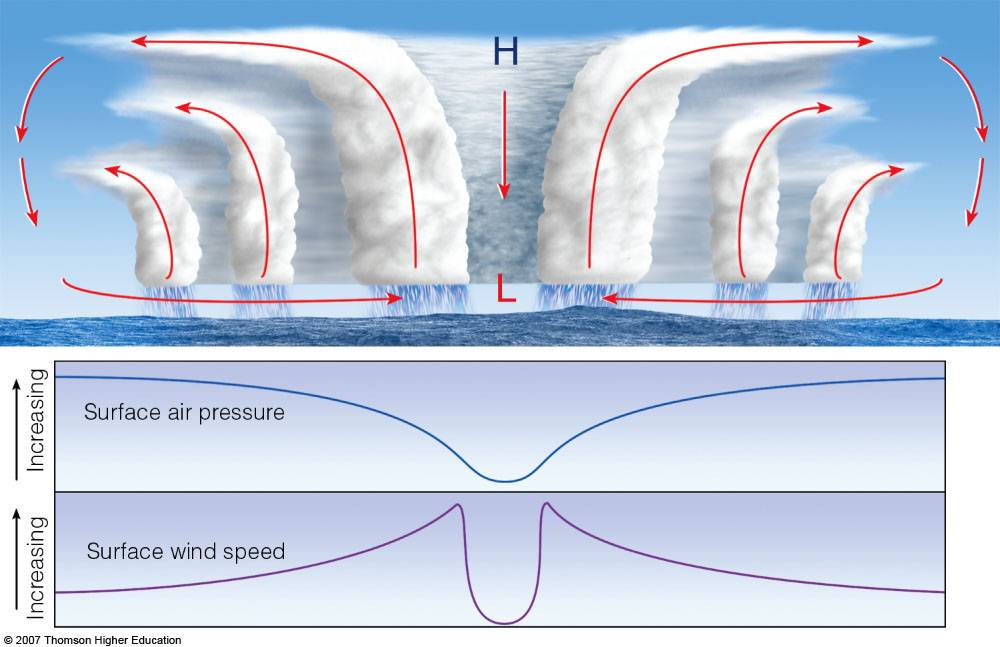
\includegraphics[width=0.9\textwidth]{hurricane_structure.jpg}\caption{Lyndon State College, 2016}\ef\FB\ect
\bct\begin{figure}[H]\ctr
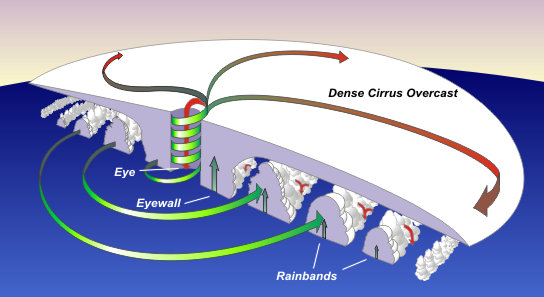
\includegraphics[width=0.9\textwidth]{hurricane.jpg}
\end{figure}\FB\ect
\begin{itemize}
  \item (颱)風眼:成熟的颱風中心多有的颱風眼,氣壓最低,風力很小,因有微弱下沉氣流,呈現少雲或無雲的狀態,下降氣流縮小增溫使溫度較周圍略高,水氣不易飽和,故無雲雨,其大小可達數十公里,強度較弱的熱帶氣旋之颱風眼常較不清楚或不存在。
  \item 眼牆:颱風中心周圍堆積高聳如牆的積雨雲,受颱風眼下沉氣流向外與往內旋入的氣流在此形成強烈輻合,是颱風內上升運動、風速及降雨最強的區域。
  \item 螺旋狀雲雨帶:渦旋狀旋轉的對流雲系(積狀雲),水平範圍約數百公里,颱風一般有500公里以上,內有垂直對流故間歇性降雨。
\item 垂直對流:成熟颱風的垂直對流高度相近,達到對流層頂附近 ,即約十幾公里高。颱風愈強,垂直對流愈強,垂直高度發展愈高,甚至略高過對流層頂。由中心往外,間或有垂直上升與下降的區域,即颱風來襲時風雨陣強陣弱的現象,較靠近中心者通常較強。
\item 外圍沉降氣流:雲雨區外圍存在外圍沉降氣流。
  \item 颱風外圍環流:指颱風七級風暴風半徑之外的風場。這些環流由於颱風的強大能量和旋轉運動而形成,水平範圍可達數百公里,攜帶大量的水氣,並導致外圍地區出現強降雨、風暴潮等天氣現象。
\end{itemize}
\sssc{高壓影響颱風路徑}
颱風路徑常受高壓帶影響,沿反氣旋方向行進。
\subsubsection{減弱消散}
颱風減弱時風速變小、中心氣壓上升。
\begin{itemize}
  \item 移入陸地:因為失去維持能量的溫暖海水,且環流受到陸地地形與摩擦力增大的破壞,而迅速減弱消散。絕大部分的強烈熱帶氣旋登陸後一至兩天即變成組織鬆散的後熱帶氣旋。但是如果能夠重新移到溫暖的洋面上,它們可能會重新發展。移經山區的熱帶氣旋可能在短期內迅速減弱。
  \item 在同一海面上滯留過久:翻起海平面30公尺以下較涼海水,熱量吸乾,使表面水溫下降,無法維持強度,熱帶氣旋因而減弱。
  \item 移入水溫低於26°C的海洋:使熱帶氣旋失去其特性(中心附近的雷暴和暖心結構),減弱為低壓區或溫帶氣旋。這是東北太平洋熱帶氣旋消散的主因。
  \item 遇上強烈垂直風切:對流組織受風切破壞。
  \item 與西風帶的作用:例如與鄰近的鋒面融合,使熱帶氣旋轉化為溫帶氣旋(稱後熱帶氣旋),這個過程會持續一至三日,在這段期間的熱帶氣旋會逐漸成為後熱帶氣旋。但就算熱帶氣旋完成轉化,很多時候仍能維持熱帶風暴的風力和一定程度的降雨。在太平洋和大西洋,由熱帶氣旋轉化而成的溫帶氣旋有時風力會達到颶風的水平,影響美國西岸或歐洲。
  \item 弱的熱帶氣旋被另一低壓區影響:受破壞而成為非氣旋性雷暴,或被另一較強的熱帶氣旋吸收。
\end{itemize}
\subsubsection{天氣型態}
\begin{itemize}
\item 螺旋狀雲雨區:潮溼且不穩定度高,易有較強降雨,地形迎風面地區易有強風豪雨,風力強勁使擴散條件較佳,與降雨洗除作用,均會使空氣品質佳;位於背風面或尚未被熱帶性低氣壓所籠罩之區域則可能發生水平風較弱、氣流過山沉降等現象,擴散條件較差,空氣品質轉差,可能有焚風。
\item 外圍沉降氣流區:在雲雨區外之區域為平均氣流沉降區,大氣普遍晴朗無雲,下沉氣流易使空氣中的汙染物易聚集在近地面聚集,垂直擴散條件不佳。此時若有汙染源排放,則汙染物易累積,使空氣品質轉差。
\end{itemize}
\subsubsection{共伴效應(Accompanied effect)}
指熱帶氣旋所挾帶之氣流遇上季風或鋒面等時產生低空輻合形成降雨的現象。
\subsubsection{藤原效應(Fujiwhara effect)/雙颱效應}
指兩個距離不遠的水旋渦或大氣旋渦(如熱帶氣旋),因為渦度、質量、相對位置的不同,而互相影響的狀態。通常以兩者連線的中心為圓心,繞著圓心互相旋轉。通常在兩或多個颱風靠近至1000公里以內時發生,除互繞外亦可能合而為一。
\subsubsection{颱風與海洋的交互作用}
\begin{itemize}
\item 颱風產生的強風有時可以將較深層的冷海水帶至海洋表面,使表面海水溫度降低。
\item 低溫海水因為無法提供足夠潛熱而不利颱風發展,因此長期停留在同一 海面的颱風強度可能會減弱。
\item 颱風可說是一種將原來低緯度熱帶海洋的熱量傳輸到大氣及中高緯度地區的天氣系統,可調節地球氣候與能量平衡。
\item 颱風中心氣壓低,將海水面吸高,當颱風登陸時常形成暴潮。
\end{itemize}
\subsubsection{侵臺颱風}
\bct\begin{figure}[H]
      \centering
      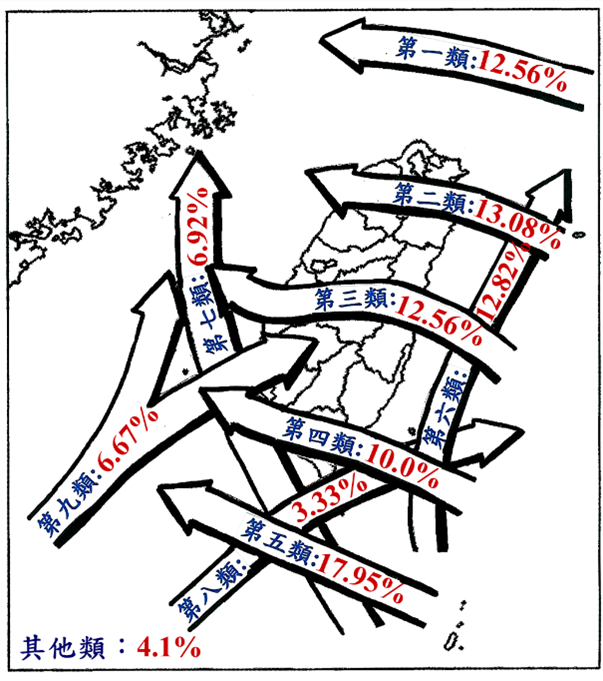
\includegraphics[width=0.7\textwidth]{fig12.png}
      \caption{侵臺颱風路徑分類圖}
  \end{figure}\FB\ect
\begin{itemize}
  \item 侵臺颱風:中央氣象署定義,颱風中心登陸臺灣,或中心未登陸,但在臺灣附近海面經過且造成路上災害的颱風,為侵襲臺灣的颱風 。
  \item 海上颱風警報:颱風暴風圈在24小時內有可能侵襲距臺澎金馬海岸線100公里範圍內之近海。
  \item 陸上颱風警報:颱風暴風圈在18小時內有可能侵襲距臺澎金馬陸地。
  \item 侵臺颱風多發源於西北太平洋(第1至8類路徑),少數來自南海(第9類路徑)。
  \item 發源於西北太平洋者形成後多受副熱帶太平洋高壓的氣流導引,沿著高壓南側朝西或西北前進。副熱帶高壓的控制減弱可能使颱風路徑受到周圍環流影響而打轉或搖擺。
  \item 侵臺颱風,由東往西者(第1至5類路徑)約占六、七成,由南往北者(第6至9類路徑)約占二成。
  \item 臺灣有高聳的山脈,颱風穿越時強度常會明顯減弱,但臺灣面積較小,無法有效切斷颱風的水氣供應使消散。
  \item 迎風面通常風雨較強;背風面通常風雨較弱,可能出現焚風。
  \item 臺灣東部沒有地形屏障,從東來的颱風對該處損害大。
  \item 颱風尾:指颱風離去途中引入西南氣流,好發於夏季,太平洋高壓勢力東退時尤甚。
  \item 西北颱:即第1類颱風路徑,從臺灣東方海面向西北進行,中心通過基隆與彭佳嶼之間海面。颱風中心未經山脈破壞,且可能引進西南氣流。其通過北部近海時使臺灣北部與西北部多吹西北風,風向垂直海岸線向內陸吹,使積水不易由河川宣洩,甚至引起淡水河海水倒灌,使大臺北地區受創嚴重。
  \item 與東北季風產生共伴效應:好發於秋冬兩季,北方的東北風南下,若臺灣附近有熱帶氣旋逼近且挾帶東南風,即易產生共伴效應,為臺灣北部及東北部地區帶來豐沛的降雨量。
\end{itemize}
\subsection{中尺度比熱差異造成的大氣系統}
\subsubsection{山風與谷風}
陸地比熱小於空氣,故白天山坡受日照溫度上升,上方空氣受熱膨脹,氣壓降低,使空氣由山谷沿山坡爬升,吹谷風;晚上山坡迅速冷卻,空氣接觸較冷的山坡而冷卻收縮,使空氣沿山坡下降,吹山風。
\subsubsection{海風與陸風}
陸地比熱小於海水,故白天受日照陸地升溫大於海水,上方空氣受熱膨脹,氣壓降低,吹海風;晚上陸地輻射冷卻快於海水,空氣冷卻收縮,吹陸風。
\subsection{季風(Monsoon)}
季風一種風向隨季節改變的現象,如亞洲(東亞)季風區、西非季風區。
\subsubsection{亞洲季風區}
東亞季風區主要成因是海陸比熱差異,但仍可能受行星風系影響,如對同向季風具有加成性、對反向季風具有抵銷性。

北半球夏季太陽輻射較強,亞洲大陸因比熱較小而快速增溫,在青藏高原、印度北部一帶形成低壓中心,風由太平洋高壓與南印度洋高壓吹向陸地,並受科氏力影響,前者在日本、朝鮮半島、中國東北一帶形成東南季風,在長江中下游一帶形成南季風,在越南、菲律賓、臺灣、閩粵一帶形成西南季風,後者在印度形成西南季風。來自海洋的季風富含水氣,受到地面加熱與地形抬升易形成積雨雲並降雨。

北半球冬季太陽輻射減弱,陸地降溫速率大於海洋,最低溫出現在西伯利亞一帶,形成蒙古—西伯利亞高壓,氣團性質屬於大陸冷氣團,季風吹向大平洋,並受科氏力影響,在中國東北、朝鮮半島、日本一帶形成西北季風,在長江中下游一帶形成北季風,在閩粵、臺灣、菲律賓、越南一帶形成東北季風,而往印度方向受青藏高原阻隔無法進入印度次大陸。該等季風原本為乾冷性質,形成乾冷天氣,如中國大陸東部地區,但若經過足夠海洋區域可能轉變為溼冷性質,易造成地形雨,如日本、臺灣、菲律賓。
\subsubsection{西非季風區}
西非季風區分布於西非幾內亞灣沿岸,主要受間熱帶輻合區季移產生,產生夏雨冬乾的氣候。

夏季時間熱帶輻合區北移至北非一帶,東南信風到達北半球後右轉,在幾內亞灣沿岸形成西南季風,因通過海洋面積大,易降雨。

冬季時間熱帶輻合區南移至幾內亞灣沿岸一帶,幾內亞灣沿岸吹東北季風,因未通過海洋而通過撒哈拉沙漠,性乾。
\subsection{臺灣夏半季常見之受亞洲綜觀大氣系統致生的天氣型態}
\subsubsection{太平洋高壓}
\begin{itemize}
  \item 太平洋高壓(籠罩):夏季副熱帶高壓籠罩時,多晴朗炎熱的好天氣。雲量少,太陽加熱使地表增溫,產生上升氣流,有助於空氣與汙染物垂直流動、混合,汙染物不易累積於近地面 。不過在太陽持續照射下,也會觸發光化反應,使白天臭氧濃度易上升並累積。
  \item 太平洋高壓邊緣:當太平洋高壓中心移動到臺灣東方或東南方上時,臺灣環境風場主要為南風或西南風,高屏空品區空氣品質較雲嘉南空品區以北良好,北部空品區位於下風處,汙染物較易累積,西南風者可能帶來水氣與乾淨空氣。
\end{itemize}
\subsubsection{西南氣流}
\begin{itemize}
  \item 西南季風:夏季盛行穩定之西南風,通常挾帶較多水氣,臺灣南部位於迎風面且易有降水現象;而北部位於下風處,汙染物易累積。
  \item 西南氣流:底層大氣有強勁的西南風,且西南風將充沛的水氣輸送至臺灣,此種暖溼氣流受中央山脈阻擋,抬升至適當高度後,其挾帶之水氣易凝結而降雨,常使中、南部地區發生豪雨。
\end{itemize}
\subsubsection{低壓帶}
低壓區內有利氣流舉升,天氣不穩定,水氣足夠時易成雲致雨。
\subsubsection{南方雲系北移}
位於南方之潮溼空氣北移,常對臺灣造成雲雨現象,常發生於梅雨季節。
\subsection{臺灣冬半季常見之受亞洲綜觀大氣系統致生的天氣型態}
\subsubsection{大陸冷高壓與東北氣流}
\begin{itemize}
  \item 高壓南下/冷高壓影響/東北季風:冬季盛行穩定之東北風,稱東北季風。在相對影響範圍較廣的西伯利亞冷高壓南下過程中,臺灣受高壓邊緣影響,附近風向常為偏北風至東北風,較北部擴散條件較佳,高屏空品區位於尾流弱風區,因此空氣品種較差,惟若風伴隨境外汙染物移入,則原擴散良好區也可能發生空氣汙染。
  \item 高壓出海:受西風帶影響,西伯利亞高壓與太平洋上的低氣壓常向東移動。當大陸高壓中心靠近華北、華中沿岸地區,且由陸地進入東海洋面時,臺灣地區以東北風為主。
  \item 高壓東移與高壓迴流:大陸冷高壓出海後,高壓中心持續向東移動,臺灣地區之環流風場由東北風轉為偏東風,而後可能轉為東南風,由於中央山脈的阻隔,臺灣西半部位於背風面,天氣較為穩定且風速較弱,擴散條件較差。高壓迴流天氣型態主要發生於秋季至隔年春季,此期間因東北季風將境外汙染物一波波移入,使得臺灣附近空氣汙染物濃度之背景值提升,而高壓迴流天氣型態又使大氣擴散條件不佳,因此每年 11 月至隔年 4 月有較多高汙染事件發生。
\end{itemize}
\subsubsection{華南雲雨區東移}
冬春之際,華南中低層大氣鋒面尚未完全通過,因暖溼空氣受冷空氣舉升產生雲雨現象,並隨著西風帶向東移動,常對臺灣造成雲雨現象。
\subsection{地球緯向(Latitudinal)行星風系(Planetary wind system)與大氣環流}
\bct\begin{figure}[H]
    \centering
    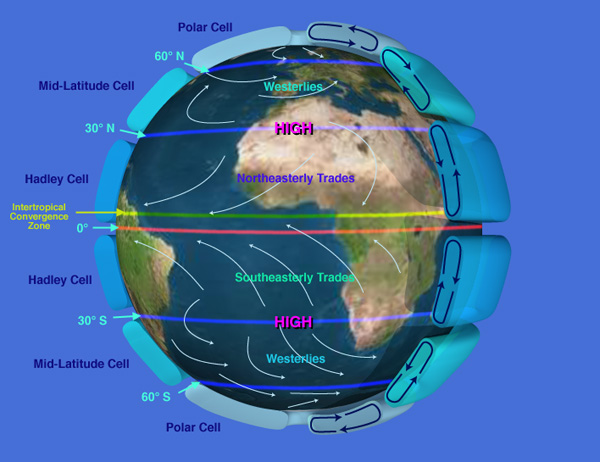
\includegraphics[width=0.9\textwidth]{circulation.jpg}
\end{figure}\FB\ect
過去以為地球的緯向大氣環流為簡單的赤道上升極地下降的單胞環流,後經驗證地球的緯向大氣環流應大致為三胞環流,但局部受到海陸性質差異、地形阻隔等原因,不同於理想情況,且地球自轉軸傾斜造成風帶季移,即環流(圈)/胞(Cells)與風帶(Wind belts)隨著季節而南北移動,北半球夏至時最北,北半球冬至時最南。

理想的三胞環流行星風系包含:
\subsubsection{哈德里環流(Hadley Cell)}
\begin{itemize}
  \item 位置:位於赤道至30度緯度(北半球和南半球各一個)。
  \item 在赤道,太陽輻射使空氣加熱並上升,形成低壓區(赤道低壓帶或赤道無風帶)。上升的空氣在高空向兩極方向流動,冷卻後在副熱帶地區(約30度緯度)下沉,形成高壓區(副熱帶高壓帶)。下沉的空氣在地表流回赤道,受到科氏力形成信風帶。
\end{itemize}
\subsubsection{費雷爾環流(Ferrel Cell)}
\begin{itemize}
  \item 位置:30度緯度至60度緯度(北半球和南半球各一個)。
  \item 特徵:費雷爾環流是由哈德里環流和極地環流的交互作用形成。地表空氣從副熱帶高壓區向極地低壓區(60度緯度)流動,在途中受到科氏力影響形成西風帶。在60度緯度,空氣上升並在高空中流回副熱帶。
\end{itemize}
\subsubsection{極地環流(Polar Cell)}
\begin{itemize}
  \item 位置:60度緯度至極地(北半球和南半球各一個)。
  \item 特徵:極地地區的冷空氣在地表流向副極地低壓區(約60度緯度),形成極地東風帶。在60度緯度,空氣上升並在高空中流回極地,形成極地高壓區。
\end{itemize}
\subsubsection{赤道低壓帶(Intertropical convergence zone, ITCZ)}
\begin{itemize}
  \item 位置:赤道附近。
  \item 特徵:氣流在此匯聚並上升,形成低壓區域。該區域通常多雲多雨。
\end{itemize}
\subsubsection{信風帶(Trade winds)}
\begin{itemize}
  \item 位置:赤道至30度緯度。
  \item 特徵:由副熱帶高壓帶向赤道流動的風。北半球的信風從東北方向吹向西南,南半球的信風從東南方向吹向西北。
\end{itemize}
\subsubsection{副熱帶高壓帶(Subtropical highs)}
\begin{itemize}
  \item 位置:約30度緯度。
  \item 特徵:穩定的高壓區域,空氣從高空下沉。
\end{itemize}
\subsubsection{西風帶(Westerlies)}
\begin{itemize}
  \item 位置:30度緯度至60度緯度。
  \item 特徵:由副熱帶高壓帶向副極地低壓帶流動的風,從西向東吹拂。
\end{itemize}
\subsubsection{副極地低壓帶(Subpolar lows)}
\begin{itemize}
  \item 位置:約60度緯度。
  \item 特徵:由暖空氣和冷空氣相遇形成的低壓區,常見暴風系統。
\end{itemize}
\subsubsection{極地東風帶(Polar easterlies)}
\begin{itemize}
  \item 位置:60度緯度至極地。
  \item 特徵:由極地高壓區向副極地低壓區流動的風,從東向西吹拂。
\end{itemize}
\subsection{沃克環流(Walker Circulation)與聖嬰-南方振盪(El Niño-Southern Oscillation, ENSO)}
沃克環流是指赤道附近沿東西方向的大氣環流模式,主要由太平洋上的海洋表面溫度(Sea surface temperature, SST)差異驅動,並與聖嬰-南方振盪密切相關。ENSO是指赤道太平洋海洋和大氣系統之間的週期性變化,其中聖嬰與反聖嬰本指東西太平洋海溫的週期性變化,南方振盪本指東西太平洋大氣氣壓週期性變化,而後發現兩者的相關性。ENSO包括兩個相反的階段:聖嬰/厄爾尼諾(El Niño)事件和反聖嬰/拉尼娜(La Niña)事件,以及中性狀態,是全球氣候變異的主要驅動因素之一。
\bct\bfH\ctr\icg[width=0.9\textwidth]{LaNina.png}\ef\FB\ect
\subsubsection{中性狀態/正常年}
\bct\begin{figure}[H]
    \centering
    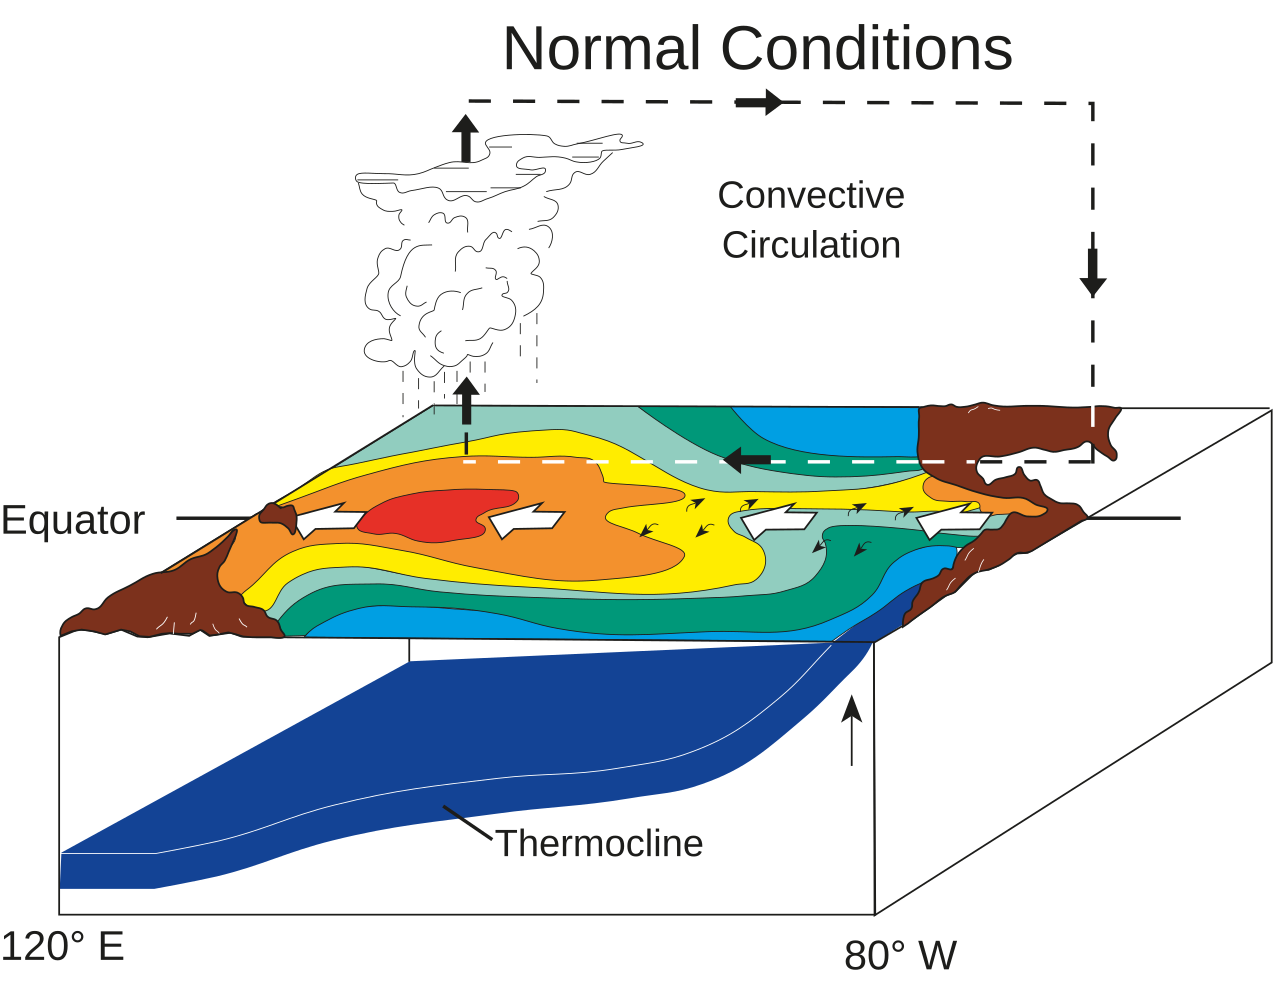
\includegraphics[width=0.9\textwidth]{normal.png}
\end{figure}\FB\ect
\begin{itemize}
  \item 地表東風:在赤道太平洋上,地表東風(東北信風與東南信風)吹拂。
  \item 赤道洋流與冷暖水區:信風因為艾克曼螺旋將溫暖的表面海水從南美洲沿岸推向西太平洋,即南赤道暖流與北赤道暖流,使西太平洋較東太平洋混合層厚、海水溫度高,在東亞海域形成西太平洋暖水區,東太平洋形成冷水區。由於西太平洋海水堆積海面高度較東太平洋高而形成赤道逆流,屬於傾斜流。
  \item 西太平洋上升氣流:溫暖的海水加熱大氣,使得西太平洋上空的空氣上升,形成低壓區。
  \item 高空西風:上升的空氣在高空中向東流動,逐漸冷卻並在東太平洋下降。
  \item 東太平洋下降氣流:在東太平洋的冷海水上空,空氣下降,形成高壓區。冷空氣在地表隨信風流回西太平洋,形成閉合環流。
  \item 秘魯湧升流:作為南太平洋暖流與北太平洋暖流的補償流,秘魯沿海發生湧升流,將深海冷水與營養物質帶到淺海,使秘魯漁場可以捕獲大量鯷魚。
\end{itemize}
\subsubsection{聖嬰事件(El Niño)/聖嬰年}
\bct\begin{figure}[H]
    \centering
    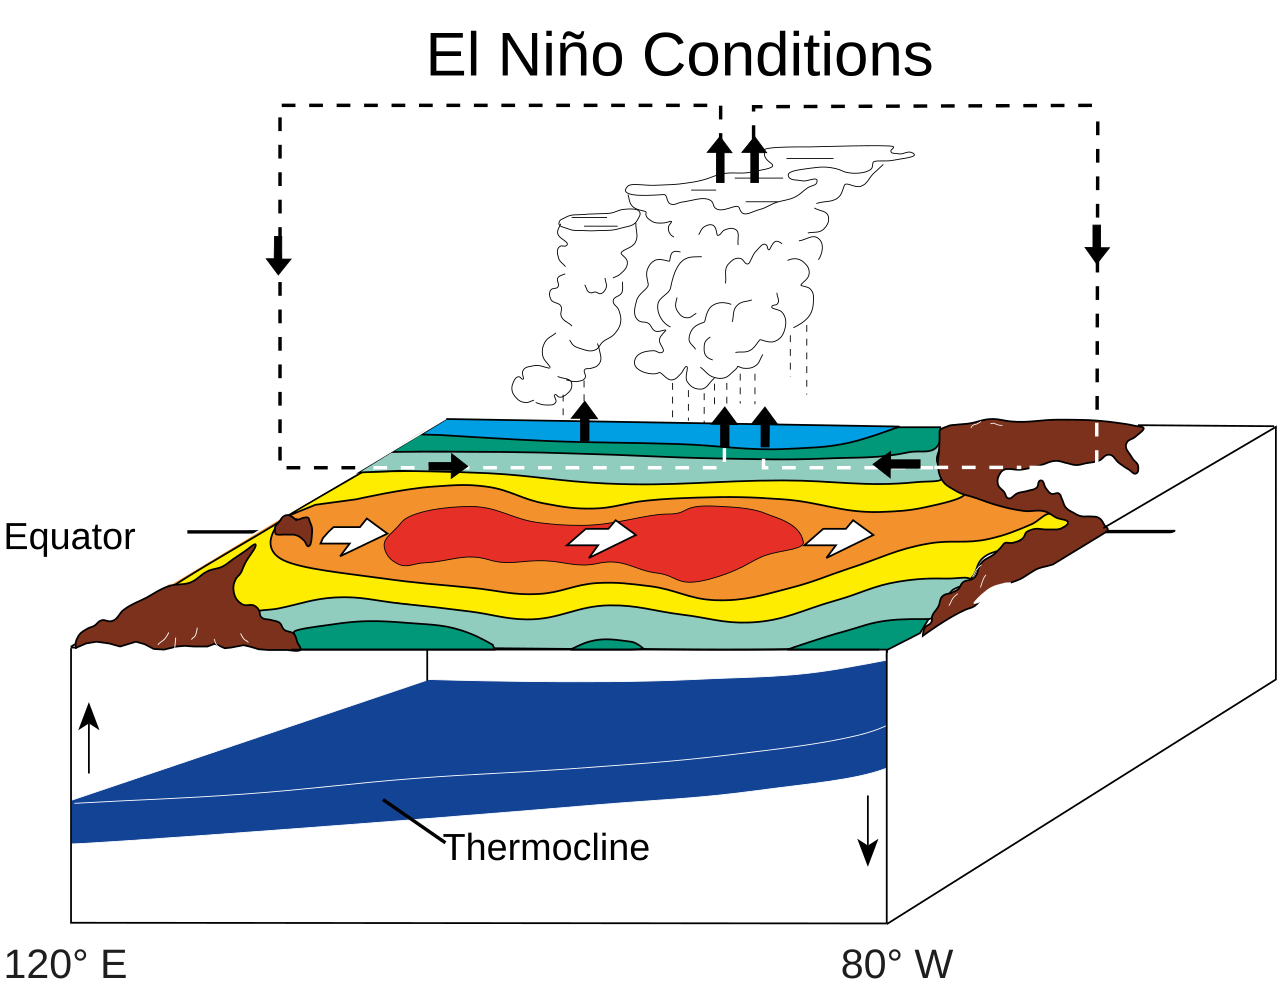
\includegraphics[width=0.9\textwidth]{Nino.png}
\end{figure}\FB
\begin{figure}[H]
      \centering
      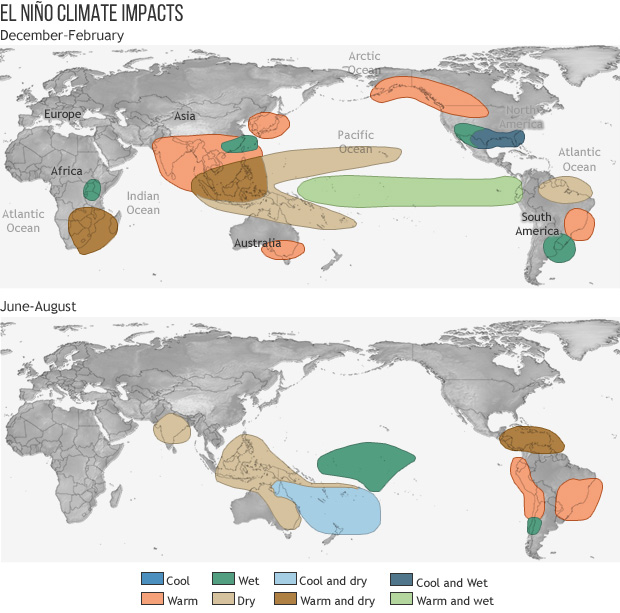
\includegraphics[width=0.9\textwidth]{NOAA_Nino.jpg}
  \end{figure}\FB\ect
\begin{itemize}
  \item 東風:東風(信風)減弱甚至逆轉。
  \item 海洋:溫暖的表面海水無法有效地被東風向西推移,導致東太平洋海水異常升溫,有時整個赤道太平洋地區海水水溫都會高於平均。東太平洋混合層增厚,西太平洋混合層變薄,秘魯湧升流減弱甚至消失,秘魯沿海湧升流減弱,帶來的營養鹽減少,表層浮游生物與葉綠素濃度減少,魚類資源與海鳥減少。
  \item 氣壓:東太平洋氣壓下降、上升氣流增加,西太平洋氣壓上升、上升氣流減少,導致沃克環流的破壞或逆轉。導致南美洲西海岸可能出現大量降雨,而澳大利亞和東南亞可能出現乾旱。
  \item 對全球氣候的可能影響:全球氣溫與海溫增高,引發低緯度海洋珊瑚白化、東南亞與西太平洋乾燥,南洋群島與澳洲森林大火、南美洲洪水、東非洪水;夏半季發生時使西太平洋颱風形成處距離歐亞大陸東岸較遠,故侵襲陸地時強度較強、印度、南洋群島與東澳氣候變乾、秘魯與巴西高原氣候變暖;冬季發生使臺灣與閩粵氣候變溼暖與春雨提早、東南亞、南亞與東亞南部氣候變暖、南洋群島氣候變乾、美國南部氣候變溼冷、北美洲西北部氣候變暖。
\end{itemize}
\subsubsection{反聖嬰事件(La Niña)/反聖嬰年}
\bct
\begin{figure}[H]
    \centering
    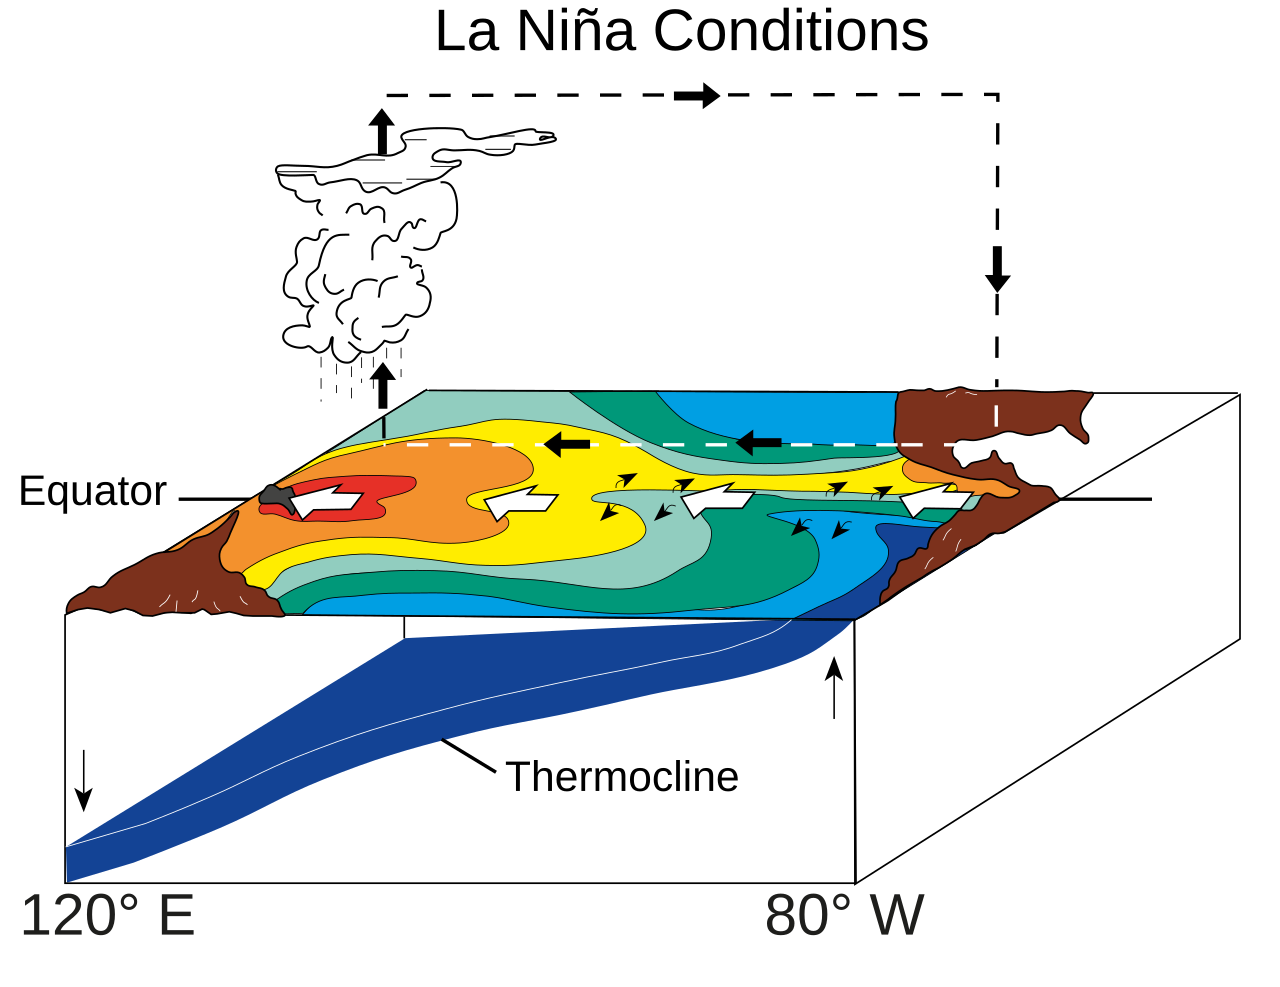
\includegraphics[width=0.9\textwidth]{Nina.png}
\end{figure}\FB
\begin{figure}[H]
    \centering
    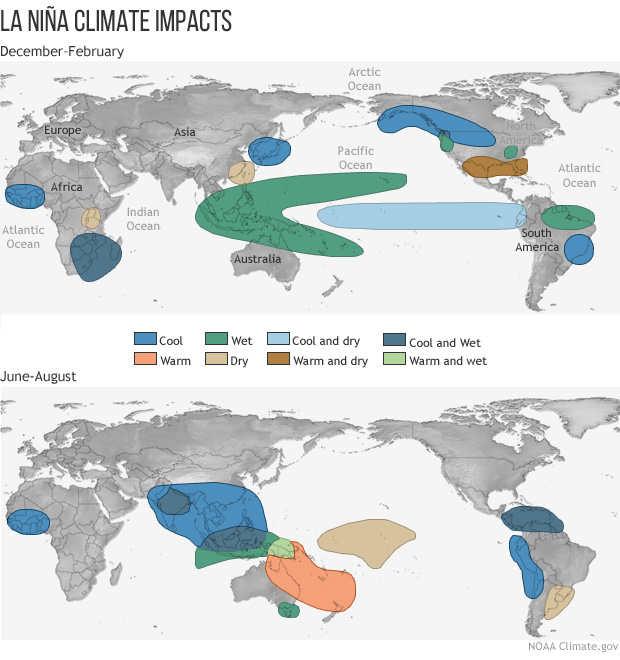
\includegraphics[width=0.9\textwidth]{NOAA_Nina.jpg}
\end{figure}\FB\ect
\begin{itemize}
  \item 東風:東風(信風)增強。
  \item 海洋:更多的溫暖海水被東風推向西太平洋,秘魯湧升流增強,東太平洋的海水異常變冷。有利於冷水魚類的生長,可能增加秘魯沿海漁業產量。
  \item 氣壓:西太平洋氣壓下降、上升氣流增強,東太平洋氣壓上升、下降氣流增強,沃克環流加強。南美洲西海岸可能出現乾旱,而澳大利亞和東南亞可能出現大量降雨。
  \item 對全球氣候可能的影響:東南亞淹水、西非變冷;夏季發生使東南亞、南亞與東亞南部氣候變冷、南洋群島氣候變溼、秘魯與加勒比海氣候變冷;冬季發生時使臺灣與閩粵氣候變乾、南洋群島氣候變溼、美國南部氣候變乾暖、北美洲西北部氣候變冷。
\end{itemize}
\section{氣象觀測與圖表}
氣象觀測可大致分為在地表或海表設立的地面觀測、利用探空氣球、投落送等方法進行的高空觀測,與利用雷達、衛星等進行的遙測。
\ssc{地面觀測}
\sssc{陸/地面觀測}
為避免阻擋,一般地面氣象觀測站設在空曠處,主要收集風向、風速、氣溫、降水量、氣壓、日照、雲量、雲狀、雲底高度等資料,常見觀測儀器如氣壓計、百葉箱、溫溼度儀、雨量儀、蒸發皿、風向風速計等。

中央氣象署現有三十個地面綜觀氣象站,除了一些目視的觀測項目如雲種與雲量外,多數已自動化;另有四百多個無人自動氣象站,觀測項目包含風向、風速、氣溫、雨量及氣壓或日照;另有一百多個只觀測雨量的無人自動雨量站。
\sssc{海面觀測}
目前海面觀測通常仰賴船舶、浮標與海上固定平臺觀測,主要觀測項目除與地面相同之項目外,另有浪高與週期等,現資料密度遠小於陸地。
\ssc{地面氣壓觀測儀器}
\sssc{福丁式水銀氣壓計(Fortin Barometer)}
\begin{itemize}
\item 水銀柱:水銀位於一端封閉、另一端浸沒在水銀槽中的玻璃管內。
\item 水銀槽與調節螺旋:水銀槽底部配有調節螺旋,用於將水銀槽的液面調整至精確的參考點,通常是槽內的象牙釘尖端。
\item 刻度尺與游標:管壁外部有刻度以測量水銀柱高度。
\item 溫度補償:福丁式氣壓計通常附有溫度計,因為水銀柱高度受溫度影響,需校正。
\end{itemize}
\sssc{空盒氣壓計(Aneroid Barometer)}
不含液體,無洩漏風險,與水銀氣壓計相比更輕、便利與耐用,但精度較低。
\begin{itemize}
\item 金屬空盒:由金屬(通常是銅或鋼)製成的薄片密封盒,內部為真空或低壓。當外界大氣壓力變化時,空盒會隨之膨脹或壓縮。
\item 彈簧或槓桿:空盒的變形通過彈簧或槓桿機構放大。
\item 指針:放大的機械位移驅動指針移動,顯示或紀錄氣壓讀數。
\end{itemize}
\subsection{地面風的觀測儀器}
一般安裝於高於周圍障礙物10公尺以上,主要觀測水平風。陣風指觀測間隔三小時內出現瞬間孟儒較平均風速大過每秒五公尺以上,其陣風風速即瞬間風速。
\subsubsection{杯式風速計(Cup anemometer)}
是一種旋轉風向風速計、速度風向風速計。由安裝在鉛直軸上的水平臂上的三或四個半球形杯組成。沿著任何水平方向流過杯子的氣流會使軸以大致與風速成正比的速率轉動。改進使可測量風向的三杯式風速計有一個標籤,當標籤順風和逆風交替移動時,杯輪的速度會增加和減少,根據這些速度的週期性變化可計算風向。
\subsubsection{風車式/螺旋槳式風向風速計(Vane anemometer)}
是一種旋轉風向風速計、速度風向風速計。由分別安裝在鉛直軸上的水平桿兩端的螺旋槳和板狀的尾部組成。風速與螺旋槳轉速略呈正比,尾部朝向風的來向。
\subsubsection{皮托管風向風速計(Pitot tube anemometer)}
是一種氣壓風向風速計。

皮托管是一根細管,一端面向氣流方向,有一個開口,測量總壓;側面有若干個小孔,稱靜壓孔,用來測量靜壓。
\begin{itemize}
\item 總壓(Total pressure):氣流正面衝擊皮托管開口,動能轉化為壓力能,測得的壓力稱為總壓。
\item 靜壓(Static pressure):氣流經過皮托管側面的小孔時,測量的壓力不受流動速度的影響,,測得的壓力稱為靜壓。
\end{itemize}
根據白努利方程,總壓等於靜壓加上動壓,動壓與流速平方成正比,即:
\[ v = \sqrt{\frac{2(P_t - P_s)}{\rho}} \]
其中:
\begin{itemize}
\item \( v \) 是流體速度
\item \( P_t \) 是總壓
\item \( P_s \) 是靜壓
\item \( \rho \) 是流體密度
\end{itemize}
缺點:對於低速流體和高湍流流體測量效果不佳。
\subsubsection{風向袋(Windsock)}
又稱風錐。是一個圓錐形紡織管,指向風向的反向,愈飽滿風速愈大。
\subsection{地面溫溼度觀測儀器}
\sssc{百葉箱(Stevenson Screen)}
一種用於保護氣象儀器(通常為溫度相關,如乾溼球溫度計、水銀最高溫度計、酒精最低溫度計)免受陽光直射、降水和其他外界干擾的設備。
\begin{itemize}
\item 外觀:通常以木製或塑料,箱體塗成白色,以反射陽光並減少吸熱。
\item 雙層結構:內外層之間有空氣層,進一步隔絕熱量。
\item 百葉:四面安裝有百葉板,以通風。
\item 安裝高度:箱底距地面1.25到2米,以避免地面輻射的影響,且地面常種植淺草。
\item 開口:開口應朝向背陽光側,如北迴歸線以北終年朝北開。
\end{itemize}
\sssc{乾溼球溫度計(Psychrometer)}
是一種用於測量空氣中溫溼度的儀器,由兩支溫度計組成。
\bit
\item 乾球溫度計為一般的溫度計,用於測量空氣的實際溫度。
\item 溼球溫度計包裹著溼布,溼布浸在水中,蒸發降溫,環境愈乾燥蒸發愈快,測量較低的溼球溫度。
\item 飽和時乾球溫度=氣溫=溼球溫度=露點。
\item 未飽和時乾球溫度=氣溫>溼球溫度>露點。
\eit
\sssc{水銀最高溫度計}
\begin{itemize}
\item 水銀:作為測溫液體,因其沸點357攝氏度、熔點-39攝氏度,適合測量高溫。
\item 窄頸:平放的毛細管內靠近水銀球的位置設有一段窄頸(節流點),當溫度升高時,水銀因膨脹被推過窄頸。當溫度下降時,窄頸阻止水銀回縮,使水銀柱保留在最高位置,紀錄期間的最高溫度。水銀柱末端的位置即為紀錄的最高溫度。
\end{itemize}
\sssc{酒精最低溫度計}
\begin{itemize}
\item 酒精:作為測溫液體,因其沸點78攝氏度、熔點-114攝氏度,適合測量低溫。
\item 浮標:平放的毛細管內有一根小玻璃浮標(指示棒)位於酒精液體中。當溫度下降時,酒精液面下降並帶動浮標下移。當溫度回升時,酒精液體上升,但浮標因內壁摩擦力保持原位,紀錄最低溫度。浮標底部的位置即為紀錄的最低溫度。
\end{itemize}
\ssc{地面雲的觀測}
觀測員目視觀測雲高、雲狀與雲量。
\subsubsection{雲高與雲狀的分類}
\begin{itemize}
\item 高雲族:形成於6000m至18000m高空。
\begin{itemize}
\item 捲雲(Ci, Cirrus):常呈現絲條狀、羽毛狀、馬尾狀、鉤狀、片狀或砧狀等。
\item 卷積雲(Cc, Cirrocumulus):似鱗片或球狀細小雲塊。
\item 卷層雲(Cs, Cirrostratus):呈現薄幕狀。
\end{itemize}
\item 中雲族:形成於2500m至6000m的高空。
\begin{itemize}
\item 高積雲(Ac, Altocumulus):呈扁圓形、瓦片狀等,且以波浪形排列。
\item 高層雲(As, Altostratus):像一種帶有條紋的幕,顏色多為灰白色或灰色。
\end{itemize}
\item 低雲族:形成於低於2500m的高空。
\begin{itemize}
\item 層雲(St, Stratus):層雲完全沒有結構,它由細小的水珠組成。層雲接地就被稱為霧。
\item 層積雲(Sc, Stratocumulus):層積雲由積雲平展而成,常呈波狀,較薄處為白色或淺灰色。
\item 雨層雲(Ns, Nimbostratus):雨層雲呈暗灰色,雲層較厚且均勻,覆蓋全天,常伴隨持續性降雨。
\end{itemize}
\item 直展雲族:有強上升氣流,故可一直從底部長到更高處,雲頂高度甚至可能略高過對流層頂。
\begin{itemize}
\item 積雲(Cu, Cumulus):積雲如同棉花團,雲體垂直向上發展,常見於上午,午間發展最旺盛,並於午後開始逐漸消散。
\item 積雨雲(Cb, Cumulonimbus):由積雲發展而來,伴隨雷暴與陣雨,雲體高聳,頂部常呈花菜狀或砧狀,雲底陰暗。
\end{itemize}
\end{itemize}
\sssc{雲量}
通常以八分量表示,指將天空分為八等分,觀測雲層遮蔽之比例,如全遮蔽計作8/8。
\ssc{地面降水觀測儀器}
降水量指無蒸發、流失或滲透等情況下,一定時間內降水儲積在一平面上,降水儲積量之深度,單位通常為毫米。測量時離地30公分以上以防濺射入內。
\sssc{虹吸式雨量儀(Siphon Rain Gauge)}
\begin{itemize}
\item 漏斗:上方的漏斗用於收集降雨,漏斗口面積固定。
\item 浮子:收集的雨水流入帶有浮子的量筒內,浮子的位移反映降水量。浮子的位移通過杠桿機構驅動紀錄筆,在時間-降水量圖上繪製連續曲線。
\item 虹吸裝置:當水位達到一定高度,虹吸裝置自動啟動,將水排出,使重置浮子位置。
\end{itemize}
\sssc{傾斗式雨量儀(Tipping Bucket Rain Gauge)}
\begin{itemize}
\item 漏斗:上方的漏斗用於收集降雨,漏斗口面積固定。
\item 傾斗:安裝在筒中軸上的小容器,兩側對稱,每側可容納一定的雨水(如0.2毫米)。一次僅一側處於承水口,當水量達到預定容量,傾斗會翻轉將水排出,並使另一側承水,並觸發電流開關使自記筆跳動一次。
\end{itemize}
\ssc{地面蒸發觀測儀器}
\sssc{A型蒸發皿(Class A Evaporation Pan)}
由直徑約1207毫米、高254毫米的不銹鋼或鋁制圓形容器組成,內部注入水,模擬自然環境中的水體蒸發,配合浮子、尺規或電子傳感器測量水面高度的變化,計算蒸發量。考慮降雨影響時,需結合雨量數據修正蒸發量讀數。
\ssc{高空觀測}
\sssc{探空氣球}
全球各測站於每國際標準時0時與12時釋放探空氣球,測量從地面到約30公里高的大氣資料,包含氣壓、氣溫、溼度、風向、風速等。觀測主要利用無線電探空儀,或稱雷文送,繫在填充氦氣的探空氣球下,以每分鐘約300至350公尺之速度上升,並以無線電回傳所記錄的資料至地面接收系統。另,以探空氣球上的GPS定位資料計算風向與風速大小。氣球上升至約30公里高時因高空氣壓過小而自行爆破,無線電探空儀隨佩掛之降落傘落下,觀測作業即結束。

中央氣象署有臺北板橋與花蓮兩測站,另有臺南永康站視需要施放,南沙島與東沙島探空站由海軍觀測,馬公、屏東、綠島由空軍氣象聯隊觀測。
\sssc{全球衛星定位式投落送}
侵臺颱風之飛機偵查及投落送觀測實驗(追風計畫)在颱風接近臺灣時以飛機直接飛到颱風周圍,從約十三公里高度投擲全球衛星定位式投落送,其中感測器、GPS 接收器與微處理器掛於拖曳傘下,每半秒回傳 GPS、氣壓、溼度與溫度資料。
\ssc{遙測}
\begin{itemize}
\item 主動遙測:主動發出電磁波或聲波等再接受被探測物反射回來的訊號。
\item 被動遙測:直接接受由被探測物發出或反射的訊號。
\end{itemize}
\ssc{雷達遙測}
雷達主要用於觀測降雨情形,觀測方法為發射微波,微波碰到降水粒子(水滴或冰晶)反射,並發生都卜勒效應,分析其回波可推測降水系統的位置與降水強度。

中央氣象署在新北市五分山、花蓮、屏東縣墾丁、臺南市七股四地各設立一座都卜勒雷達(Doppler radar)站。
\sssc{臺灣實驗性大氣移動雷達(Taiwan Experimental Atmospheric Mobile-Radar TEAM-R)}
可移動至各種地形,具有都卜勒與雙偏極化兩功能,後者指發射分別平行與垂直地面偏極化(偏振)方向的電磁波觀測,因為愈大的水滴降落時遇到越大的阻力,形狀愈扁,平行地面方向投影面積大於垂直地面方向,反之,小水滴形狀較圓,平行地面方向投影面積約等於垂直地面方向。
\sssc{雷達合成回波圖(Composite reflectivity)}
\bct\bfH\ctr\icg[width=0.8\tw]{CV1.png}\ef\FB\ect
\ssc{人造衛星遙測}
主要由氣象衛星在高空接受雲反射的可見光與雲所輻射的紅外線,可偵測雲層、鋒面、颱風、雷雨等。

氣象衛星多為同步衛星或繞極衛星:
\begin{itemize}
\item 同步衛星:離地約三萬六千公里高,始終在一地上空,解析度較差,拍攝範圍較大。
\item 繞極衛星:離地約八百多公里高,經南北極經向繞行,每日繞地14.25圈,可經過全球,解析度較佳,拍攝範圍較小。
\end{itemize}
\subsubsection{紅外線衛星雲圖}
利用衛星上之紅外線儀器,來測量雲層的溫度。溫度低的雲層會以亮白色顯示,表示此處的雲頂較高;溫度高的雲層會以暗灰色顯示,表示此處的雲頂較低。
\subsubsection{可見光衛星雲圖}
利用雲頂反射太陽光的原理拍攝,故僅能於白晝進行攝影。較厚的雲層反射能力較強,會顯示出亮白色;較薄的雲層反射能力較強,會顯示出暗灰色。
\subsection{天氣圖(Weather (analysis) chart)}
天氣圖分為地面天氣圖與不同高度的高空天氣圖。

地面天氣圖以海平面為基準,將觀測站觀測資料填在地圖上而得,若地表非位於海平面,則換算至海平面。

天氣符號可分為測站觀測資料與天氣系統,前者如風向、風速、溼度、溫度、氣壓、雨量等,後者如等壓線、鋒面、颱風等。

另有結合衛星雲圖與地面天氣圖的複合式地面天氣圖以利閱讀,但少了測站觀測資料。
\bct\begin{figure}[H]\ctr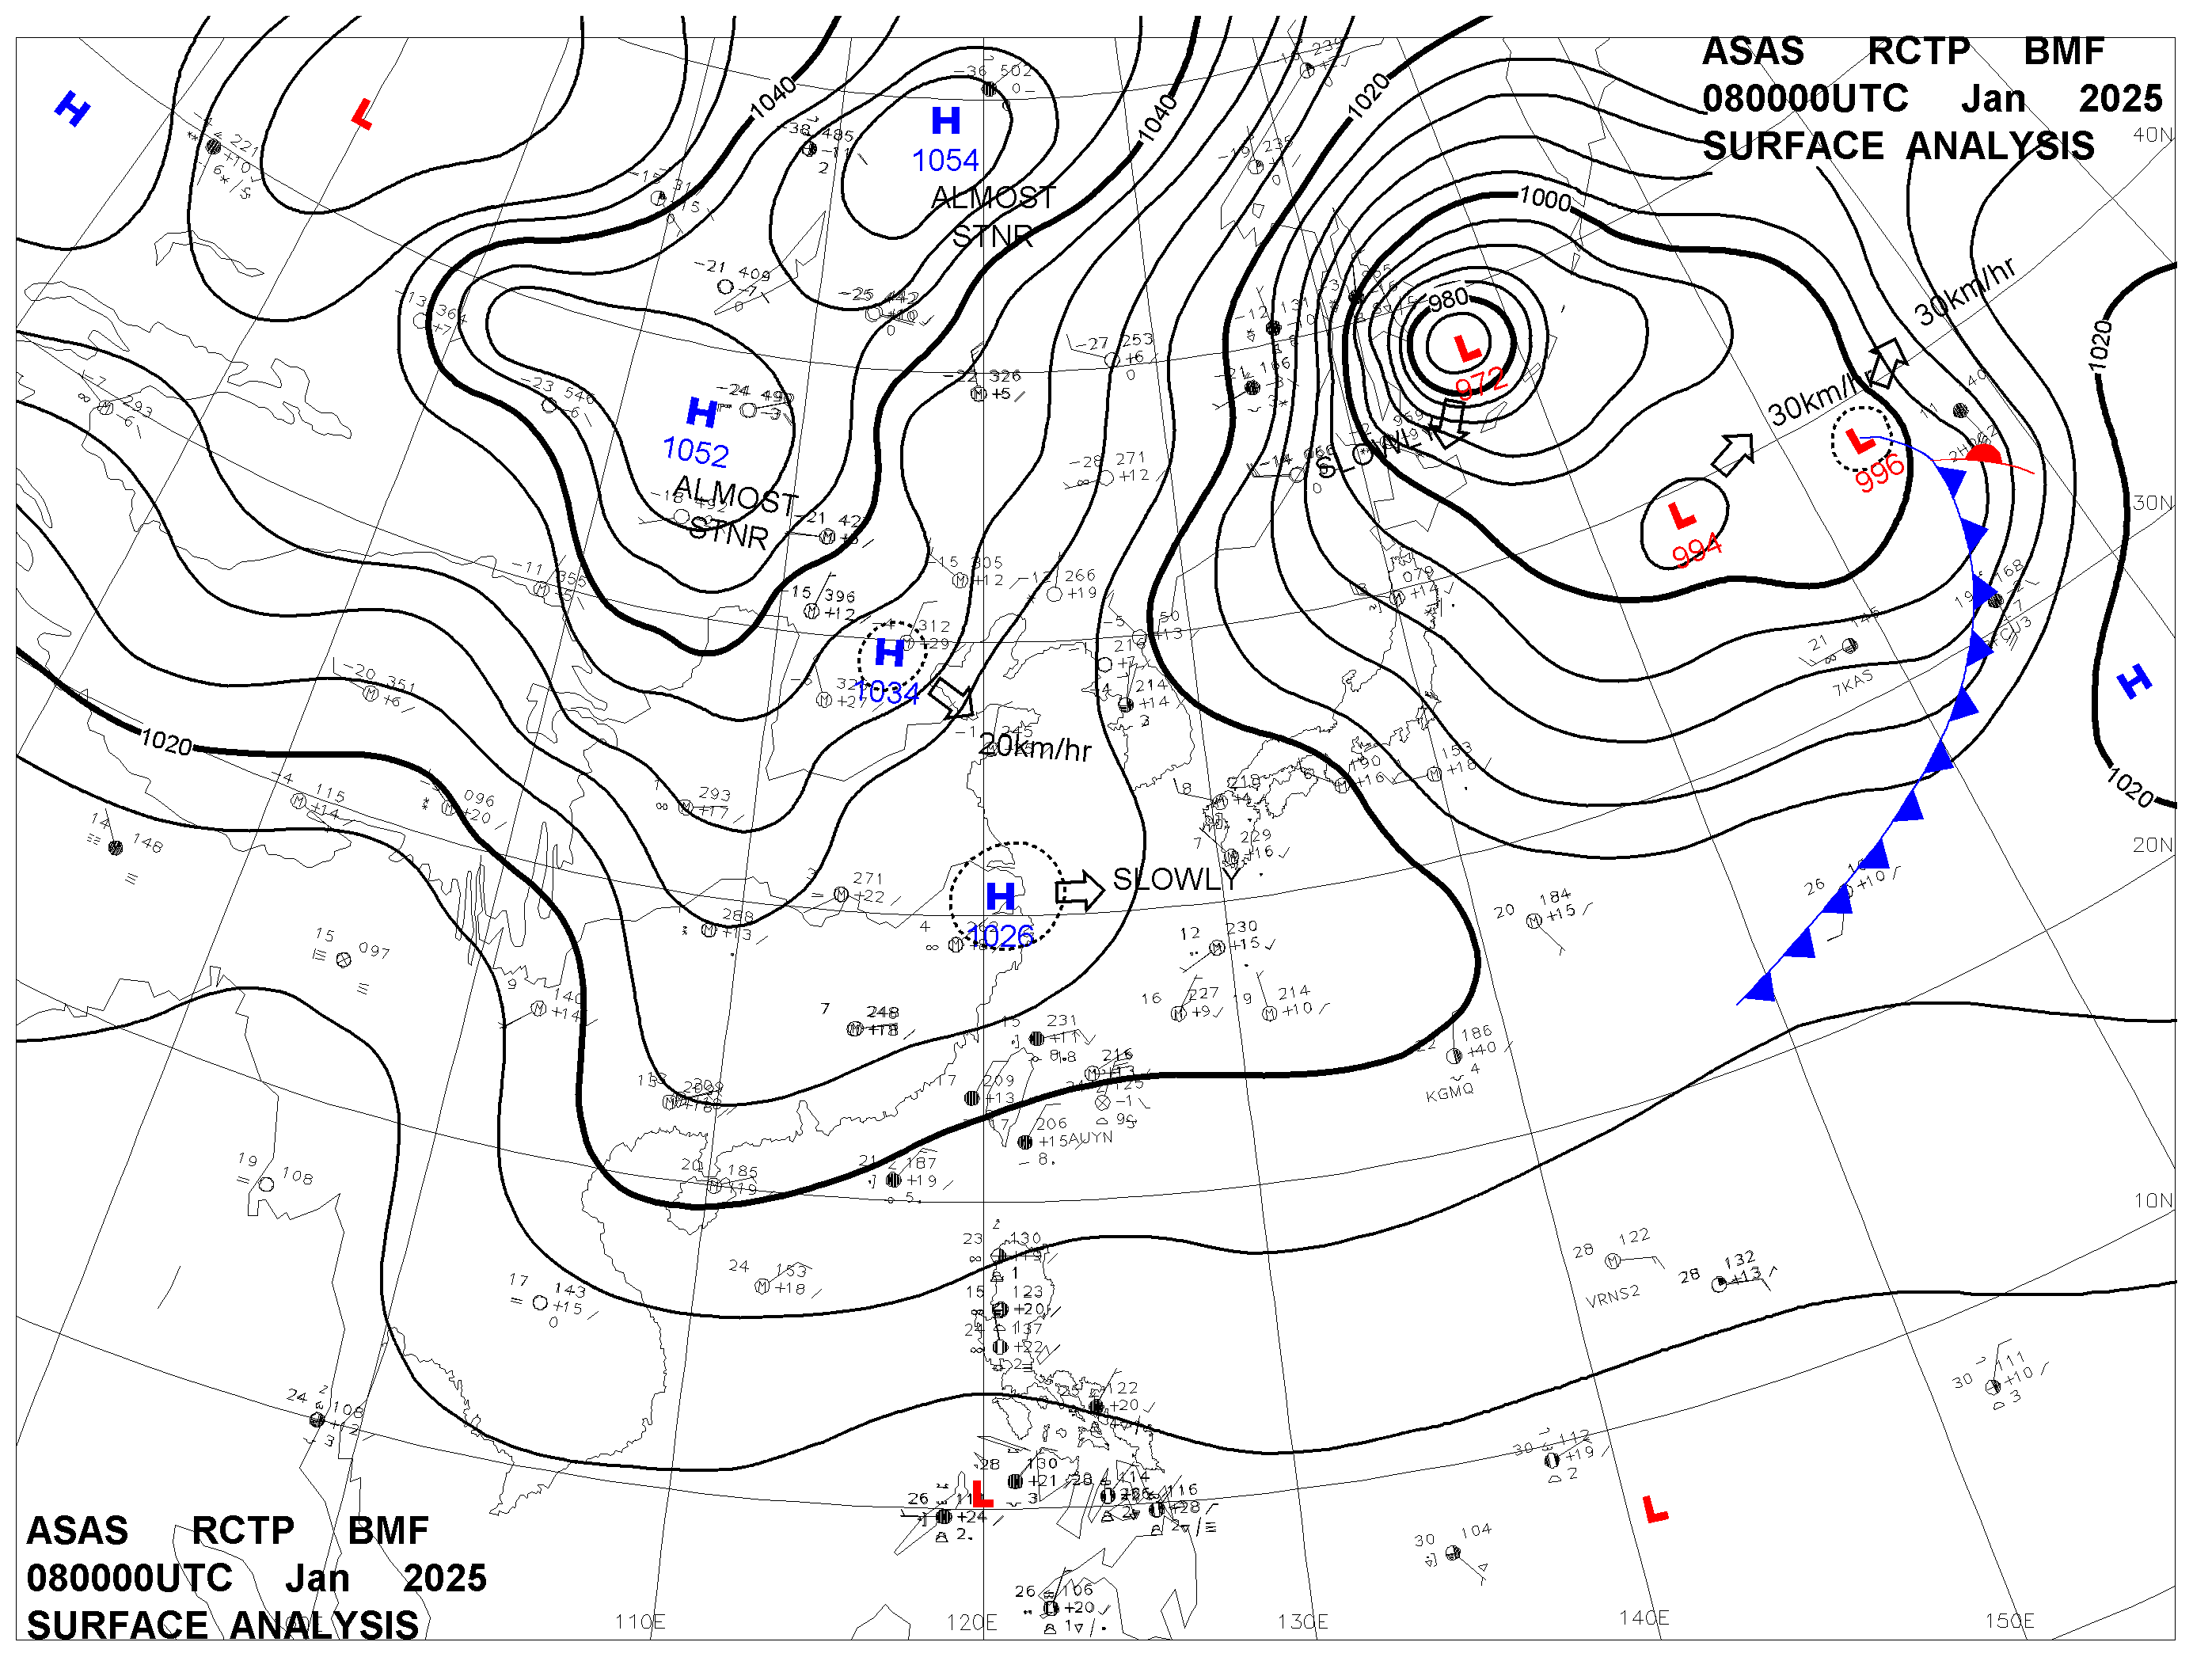
\includegraphics[width=0.9\textwidth]{FI04.png}\caption{地面天氣圖}\end{figure}\FB\ect
\sssc{測站符號(Station symbol)}
風旗的中心為一圓,其中表雲量(Sky/cloud cover),一長直線自圓周上延伸指向風的來向,其上若干三角旗或線條表風速(節),左上數字表氣溫(攝氏度),左下數字表露點(攝氏度),左中或測得位置符號(如有)表現在天氣(Present weather),天氣符號(如有)之左數字(如有)表能見度(Visibility)(英里),下方符號表雲高雲種(Cloud),右上數字為氣壓(百帕),右下數字(如有)表降水量(毫米),右中數字表三小時內氣壓變化(百帕),氣壓變化數字右之符號表氣壓趨勢(Pressure trend)。
\bct\begin{figure}[H]\ctr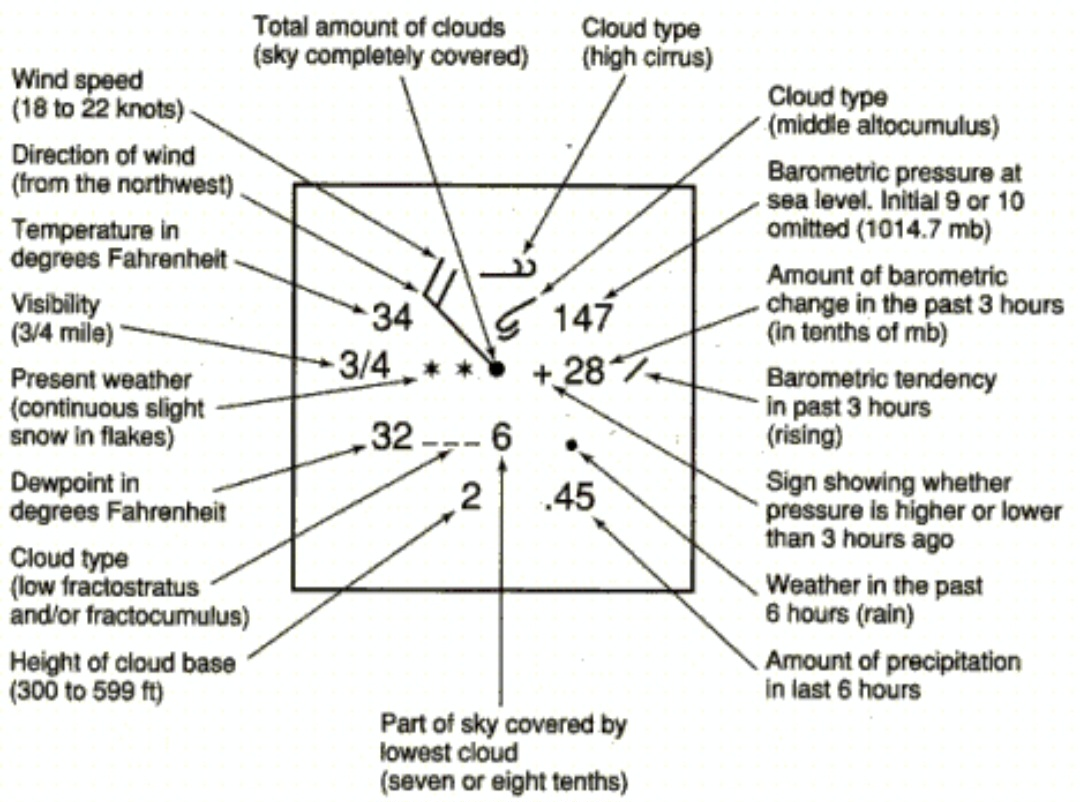
\includegraphics[width=0.9\textwidth]{station_symbol.jpg}\end{figure}\FB\ect
\begin{itemize}
\item 風速符號:節(Knot)表海哩每小時,一海哩約1.872公里。三角旗(Pennant/flag)表50節,長線(Long barb)表10節,短線(Short barb)表5節。把所有三角旗與線條所代表的速度加總為風速。
\item 雲量符號:
\bct\begin{figure}[H]\ctr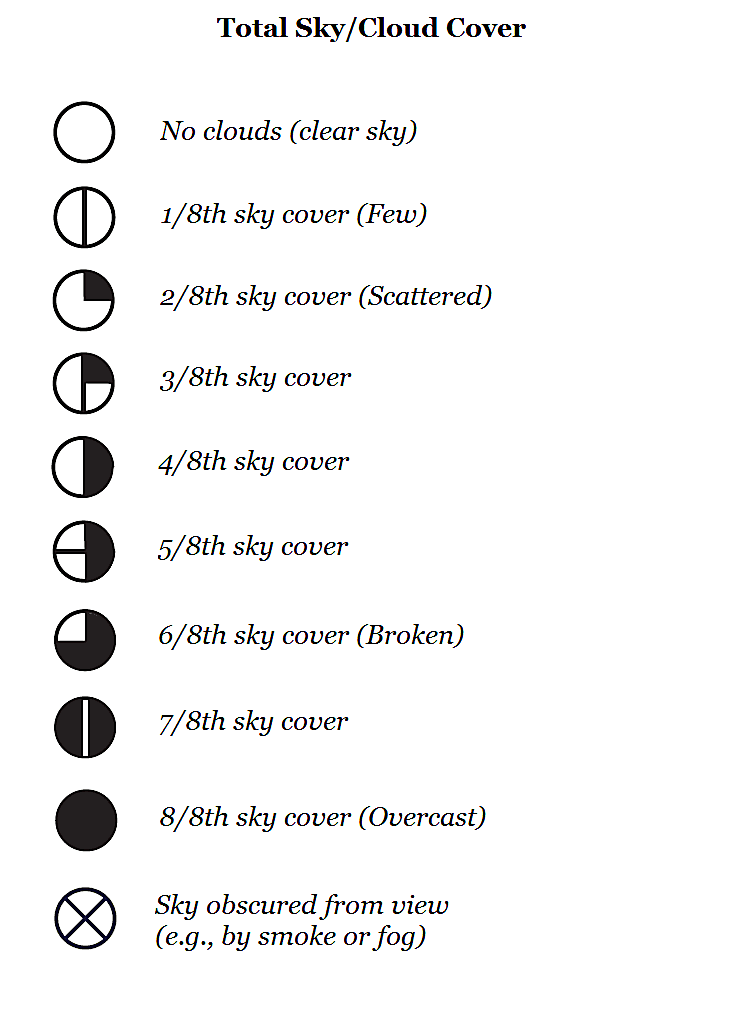
\includegraphics[width=0.6\textwidth]{sky.png}\caption{Tiffany Means, 2024. \href{https://www.thoughtco.com/symbols-on-weather-maps-3444369}{https://www.thoughtco.com/symbols-on-weather-maps-3444369}.}\end{figure}\FB\ect
\item 氣壓符號:10ab.c 百帕與 9ab.c 百帕均記作 abc。
\item 雲高雲種符號:
\bct\begin{figure}[H]\ctr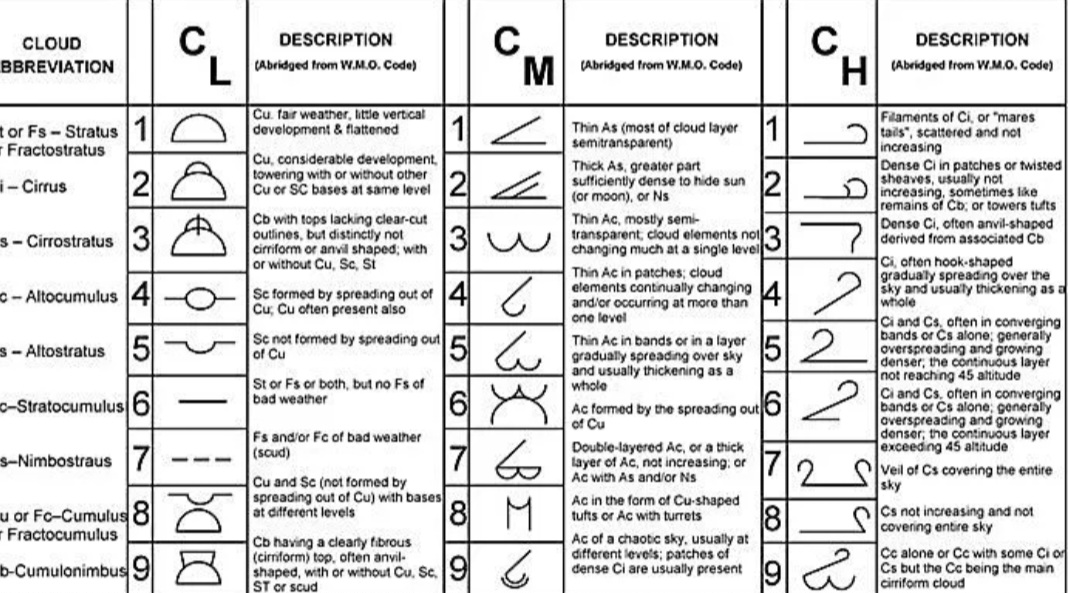
\includegraphics[width=0.9\textwidth]{cloud.jpg}\caption{Tiffany Means, 2024. \href{https://www.thoughtco.com/symbols-on-weather-maps-3444369}{https://www.thoughtco.com/symbols-on-weather-maps-3444369}.}\end{figure}\FB\ect
\item 現在天氣符號:
\bct\begin{figure}[H]\ctr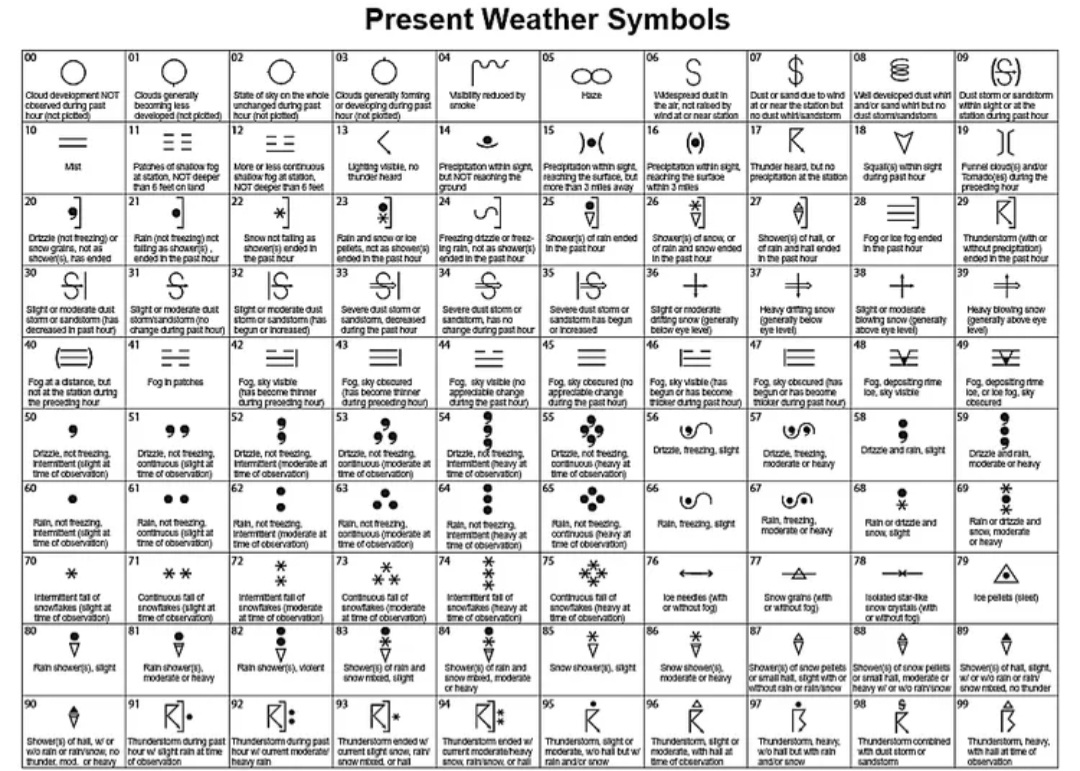
\includegraphics[width=0.9\textwidth]{weather.jpg}\caption{Tiffany Means, 2024. \href{https://www.thoughtco.com/symbols-on-weather-maps-3444369}{https://www.thoughtco.com/symbols-on-weather-maps-3444369}.}\end{figure}\FB\ect
\item 氣壓趨勢符號:
\bct\begin{figure}[H]\ctr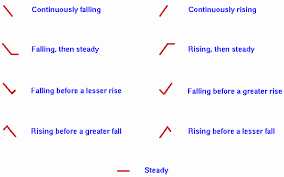
\includegraphics[width=0.6\textwidth]{trend.png}\end{figure}\FB\ect
\end{itemize}
\sssc{氣壓}
等壓線為測得相同氣壓之各點之圓滑連線,兩條等壓線之間隔通常固定為4hPa,數值以能被4整除為原則。

高氣壓標為藍色H,下或標最高氣壓;低氣壓標為紅色L,下或標最低氣壓。
\sssc{鋒}
\bct\begin{figure}[H]
    \centering
    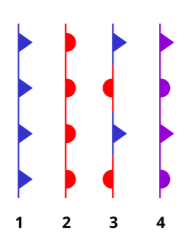
\includegraphics[width=0.9\textwidth]{front.png}
    \caption{
1. 冷鋒\\
2. 暖鋒\\
3. 滯留鋒\\
4. 囚錮鋒
}
\end{figure}\FB\ect
\sssc{熱帶氣旋}
\begin{itemize}
\item 熱帶低壓:紅色(或不計顏色)圓形內一X形,下或一 T.D.,下或標最低氣壓。
\item 輕度颱風:藍色(或不計顏色)空心颱風形,下或標最低氣壓。颱風形指上6下9共用圓形之圖形。
\item 中度颱風:綠色(或不計顏色)實心颱風形,下或標最低氣壓。
\item 重度颱風:紅色(或不計顏色)實心颱風形,下或標最低氣壓。
\end{itemize}
\section{天氣預報(Weather forecast)}
天氣預報是依據過去與現在已知的天氣狀況來預測未來的天氣,目前的天氣預報通常為數值天氣預報,指通過將數據化的氣象觀測資料輸入高速電腦進行數值分析所得之預測。
\ssc{天氣預報的限制}
\begin{itemize}
\item 氣象觀測資料不足:目前各國探空站約相隔四百至五百公里,中小型大氣系統如龍捲風、熱對流形成的雷雨胞等無法觀測到。
\item 數值分析準確度不足:目前一般天氣預報在十日之外準確度不高。
\item 電腦運算能力:今電腦運算能力高,可高速運算。
\end{itemize}
氣象預報的理論極限稱可預報度。較大尺度的系統通常可在較長時間前做出預報,雷雨、龍捲風等較小尺度者可做出預報的期限通常較短。
\end{document}